\documentclass[11pt,a4paper]{article}
\usepackage[T1]{fontenc}
\usepackage[utf8]{inputenc}
\usepackage{amsmath,amssymb,amsthm,mathtools}
\usepackage{geometry}
\usepackage{hyperref}
\usepackage{microtype}
\usepackage{tikz}
\usetikzlibrary{positioning,arrows.meta}
\usepackage{booktabs}
\usepackage{array}
\geometry{margin=2.5cm}

\theoremstyle{definition}
\newtheorem{definition}{Definition}[section]
\theoremstyle{plain}
\newtheorem{theorem}{Theorem}[section]
\newtheorem{lemma}[theorem]{Lemma}
\newtheorem{proposition}[theorem]{Proposition}
\newtheorem{corollary}[theorem]{Corollary}
\theoremstyle{remark}
\newtheorem{remark}[theorem]{Remark}
\newtheorem{example}[theorem]{Example}
\DeclareMathOperator{\Tr}{Tr}
\DeclareMathOperator{\Herm}{Herm}
\newcommand{\Det}{\mathsf{Det}}
\newcommand{\Comb}{\mathsf{Comb}}
\newcommand{\affdim}{\dim_{\mathrm{aff}}}
\newcommand{\id}{\mathrm{id}}
\newcommand{\SDet}{\mathsf{SDet}}
\newcommand{\concat}{\mathbin{\|}}

\title{\textbf{Quantum Combs, Higher-Order Processes, and the Normalization-Defect (Intercept) Principle}}
\author{Amin Abaee\\
\small Email: \href{mailto:amin_abaee@ut.ac.ir}{amin\_abaee@ut.ac.ir}\\
\small Independent Researcher\\
\small ORCID: 0000-0002-0019-1842}
\date{}

\newcommand{\keywords}{\noindent\textbf{Keywords:} Quantum combs; higher-order processes; superchannels; normalization constraints; affine dimension; environment decoration; categorical adjunctions; quantum error correction.}

\begin{document}
\maketitle

\begin{abstract}
We define the finite-dimensional one-slot deterministic superchannel
category directly by its normalized two-tooth Choi operators and define
an explicit environment-decoration map on Choi normal forms by
identity-wire insertion. A right adjoint to such decoration would
internalize the environment universally, as a currying operation on
processes. The primary result is an affine nonrepresentability theorem;
we then show that any affine endofunctor extending this map has no right
adjoint, and a dual tester-dimension argument that it has no left adjoint. For an input channel type $A\to B$ and an output
channel type $C\to D$, the affine dimension of the hom-set is
\[
d_C^2(d_A^2-1)+d_C^2d_A^2d_B^2(d_D^2-1).
\]
Writing $u=d_A^2$, $v=d_B^2$, this is
\[
\alpha_Cuv+\beta_Cu-\beta_C,
\qquad \alpha_C=d_C^2(d_D^2-1),\quad \beta_C=d_C^2.
\]
Normalization thus ties the constant term rigidly to the source-linear
coefficient; we call this rigidity the normalization-defect (intercept)
principle. Environment decoration sends $(u,v)$ to $(eu,ev)$, where
$e=d_E^2$, and hence sends this polynomial to
\[
e^2\alpha_Cuv+e\beta_Cu-\beta_C,
\]
rescaling the source-linear coefficient while leaving the constant term
fixed.
Any right-adjoint representing object $GY=(C',D')$ has the same normalization
relation between its $u$ coefficient and constant term: its source-linear
coefficient equals its first-target-input squared dimension,
$\beta_{GY}=d_{C'}^2$. Equality of affine dimensions with the decorated
hom-sets on all sources would therefore force $\beta_{GY}=\beta_C$ and
$\beta_{GY}=e\beta_C$, so $e=1$. Thus the
environment-decoration functor has no right adjoint when $d_E>1$.
A dual evaluation at the trivial channel object forces
$d_P^2=e^2-e+1$, strictly between consecutive squares, and excludes every
left adjoint as well.
These obstructions imply that the canonical parallel tensor product on
the category is not closed at nontrivial environment objects.
The obstruction is universal: it excludes a representing object uniform
over all sources and is consistent with the recoverability of individual
processes.
The theorem is stated for the one-slot deterministic superchannel
category and is extended, in an appendix, to the category of
deterministic combs of arbitrary finite order, where environment
decoration is shown to have neither adjoint at any order; the auxiliary
sequential-body calculation appears in a further appendix.
\end{abstract}

\keywords

\section{Introduction}

Quantum combs provide a finite-dimensional framework for sequential quantum networks and higher-order transformations of quantum operations \cite{chiribella2008,chiribella2009,chiribella2013}. They describe processes with open channel slots, memory systems, and a prescribed causal order. This makes them a natural setting in which to ask whether an external environment can be internalized universally at the level of higher-order processes. The fixed-order setting is distinct from process-matrix approaches to indefinite causal order \cite{oreshkov2012} and is developed here entirely in finite dimensions, with standard quantum-information conventions \cite{watrous2018}.

The question studied here is categorical. Fix a finite-dimensional Hilbert space $E$ and let $T_E$ decorate the Choi normal form by identity environment wires. We ask whether $T_E$ has a right adjoint in the one-slot deterministic superchannel category $\SDet$, in the usual categorical sense of adjunctions \cite{macLane1998}. Such a right adjoint would provide a universal currying operation: every process whose input carries an environment would be represented by a process on the original system alone, naturally and uniformly over all source objects in $\SDet$.

The answer is negative for $d_E>1$. The proof is based on affine dimensions of normalized comb sets. The exact obstruction depends on the causal convention. For the standard superchannel convention, an input channel $A\to B$ inserted into an output channel $C\to D$ has body teeth $(C,A)$ and $(B,D)$. Its dimension is
\[
 d_C^2(d_A^2-1)+d_C^2d_A^2d_B^2(d_D^2-1).
\]
With $u=d_A^2$ and $v=d_B^2$, this is
\[
 \alpha uv+\beta u-\beta.
\]
The normalization constraint rigidly identifies the coefficient of $u$ with the negative of the constant term. Environment decoration sends $(u,v)$ to $(eu,ev)$, where $e=d_E^2$. It changes the $u$ coefficient but leaves the constant term fixed. No representing object can satisfy both requirements unless $e=1$. A dual tester-dimension argument excludes a left adjoint as well: adjointability at the trivial object $(\mathbb C,\mathbb C)$ would force $p=e^2-e+1$, strictly between consecutive squares. The decoration functor therefore has
neither adjoint when $d_E>1$. Neither obstruction is an artefact of the
one-slot convention: in the category of deterministic combs of
arbitrary finite order constructed in Appendix~\ref{app:allorders},
the same environment decoration has neither adjoint at any order.

We refer to this normalization-coefficient obstruction as the \emph{intercept principle}. In an auxiliary sequential-body convention, the dimension polynomial has the form $(1+S)uv-u$, with $S$ the sequential-body sum defined in Appendix~\ref{app:seqbody}, and the $v$-intercept is scaled by environment decoration. This sequential-body calculation is auxiliary and does not enter the definition of the standard superchannel hom-set.

The result concerns functorial adjointability, not individual invertibility. An individual comb may admit a recovery operation, a code-subspace correction, or a state-dependent Petz map. What fails is a universal right-adjoint representation for all source objects of $\SDet$. The result is also not a thermodynamic arrow theorem; monoidal closedness is settled for the canonical parallel tensor product in Section 6.

\paragraph{Reader's guide.} Section 2 defines the one-slot category $\SDet$ by normalized two-tooth Choi operators and fixes the typed link product. Section 3 defines the object decoration and its Choi morphism map and verifies functoriality. Section 4 proves the affine-dimension formula, the unconditional affine
nonrepresentability theorem, the no-right-adjoint theorem for $T_E$, and
the corollary for arbitrary affine endofunctors with the same object part,
together with the dual no-left-adjoint theorem and its corollary.
Section 5 develops toy models for deterministic channels and finite classical stochastic maps, compares the obstruction with instruments, CPM, and quantum error correction, discusses the one-slot restriction and multi-slot extensions, and collects the summary tables. Section 6 constructs the canonical parallel tensor product on $\SDet$ and shows that it is not closed. Section 7 states the scope, and Section 8 concludes. The appendices record the auxiliary sequential-body construction, causal placements and link-product conventions, the detailed component and normalization verifications, and the pointwise instrument obstruction. Appendix~\ref{app:allorders} constructs the category of comb types of arbitrary finite order and extends both adjunction obstructions to the full hierarchy.

\section{Standard one-slot deterministic superchannels}

All Hilbert spaces are finite-dimensional, nonzero, and complex. We use the
unnormalized Choi convention of Choi and Jamio\l{}kowski
\cite{choi1975,jamiolkowski1972}:
\[
J(\Phi)=(\id\otimes\Phi)(|\Omega\rangle\langle\Omega|),
\qquad |\Omega\rangle=\sum_i|i\rangle\otimes|i\rangle.
\]
Thus $\Phi:X\to Y$ is CPTP exactly when
\[
J(\Phi)\ge0,
\qquad \Tr_YJ(\Phi)=I_X.
\]

\paragraph{Strict tensor convention.}
We work in a strictified category of finite-dimensional Hilbert spaces
with fixed ordered tensor products. Associators and symmetry maps are
suppressed. If one does not strictify, every equality below is understood
up to the corresponding canonical unitary coherence isomorphism; such
permutations preserve positivity, normalization, and affine dimensions.
The construction is based on chosen Choi bases. Changing those bases
conjugates all Choi operators by canonical unitaries and preserves
positivity, normalization, affine dimensions, and affine bijections; the
no-go result is therefore independent of the chosen bases.

\begin{remark}[Skeleton]
It is harmless to replace $\SDet$ by a skeleton whose objects are pairs of
positive integers $(m,n)$, represented by $\mathbb C^m,\mathbb C^n$ with
standard bases. Then $u,v$ range literally over $\{1,4,9,\ldots\}$.
\end{remark}

\begin{definition}[Standard one-slot deterministic superchannel category]
\label{def:SDet}
Let $\SDet$ be the category whose objects are ordered pairs
\[
X=(X_0,X_1),
\]
interpreted as channel types $X_0\to X_1$. For objects
$X=(A,B)$ and $Y=(C,D)$, a morphism $F:X\to Y$ is a positive operator
\[
R_F\in\Herm(C\otimes A\otimes B\otimes D)
\]
for which there exists a unique auxiliary prefix operator
\[
R_F^{(1)}\in\Herm(C\otimes A)
\]
satisfying
\[
\Tr_A R_F^{(1)}=I_C,
\qquad
\Tr_D R_F=I_B\otimes R_F^{(1)}.
\]
The second equation uses the fixed canonical permutation from
$C\otimes A\otimes B$ to $B\otimes C\otimes A$. The tensor order
$C,A,B,D$ is part of the definition. Equivalently,
\[
R_F^{(1)}=\frac{1}{d_B}\Tr_{BD}R_F,
\]
which follows by tracing the second normalization equation over $B$.
\end{definition}

Standard deterministic-superchannel
realization theorems identify these operators with fixed-order
circuit-with-holes superchannels \cite{chiribella2009,chiribella2013};
circuits are used below only as intuition. The canonical body order is
illustrated in Figure~\ref{fig:SDet-body}. Alternative hole placements
define different typed process categories rather than additional morphisms of
$\SDet$; the alternative placements are compared in
Appendix~\ref{app:placements}.

\begin{definition}[Typed link product and composition]
\label{def:typed-link}
Let
\[
R_F\in\SDet((A,B),(C,D)),
\qquad
R_G\in\SDet((C,D),(P,Q)).
\]
Use the fixed Choi ordering $C,A,B,D$ for $R_F$ and
$P,C,D,Q$ for $R_G$. Define the named permutation unitaries
\[
U_F:C\otimes A\otimes B\otimes D\to C\otimes D\otimes A\otimes B,
\]
\[
U_G:P\otimes C\otimes D\otimes Q\to P\otimes Q\otimes C\otimes D,
\]
and let $U_{\mathrm{out}}:P\otimes Q\otimes A\otimes B\to
P\otimes A\otimes B\otimes Q$ be the declared output permutation. Put
\[
\widehat R_F:=I_{P\otimes Q}\otimes(U_FR_FU_F^\dagger),
\qquad
\widehat R_G:=(U_GR_GU_G^\dagger)\otimes I_{A\otimes B},
\]
with both operators regarded on the explicitly ordered total space
$P\otimes Q\otimes C\otimes D\otimes A\otimes B$ after the displayed
embeddings. Define
\[
R_{G\circ F}:=\operatorname{Link}_{C,D}(R_G,R_F),
\]
where
\[
\operatorname{Link}_{C,D}(R_G,R_F):=
U_{\mathrm{out}}\operatorname{Tr}_{C\otimes D}
\left[\widehat R_G^{\,T_{C\otimes D}}\widehat R_F\right]
U_{\mathrm{out}}^\dagger.
\]
Here the partial transpose is taken in the fixed Choi bases on the linked
factors. The displayed embeddings make the operator multiplication
well-defined on the total space $P\otimes Q\otimes C\otimes D\otimes A\otimes B$. All
compositions in the main text and the appendices use this convention.
\end{definition}

\begin{remark}[Component form of composition]
Expanding the displayed permutations and partial transpose in the fixed
oriented Choi bases gives the component contraction used below:
\[
(R_{G\circ F})_{pabq,p'a'b'q'}
=\sum_{c,c',d,d'}
(R_G)_{pcdq,p'c'd'q'}(R_F)_{cabd,c'a'b'd'}.
\]
Indeed, $U_F$ moves the $D$ factor next to $C$ and $U_G$ moves the $Q$
factor next to $P$; the partial transpose exchanges the two linked
indices in each of $C,D$, and the trace identifies the linked primed and
unprimed indices. The final $U_{\mathrm{out}}$ restores the order
$P,A,B,Q$. If a different Choi orientation is selected, the same
calculation produces the corresponding crossed indices; the operator-level
definition above is primary. The underlying index calculation is recorded
in Appendix~\ref{app:component-link}.
\end{remark}

For any explicitly specified collection $S$ of matching tensor factors,
$X*_S Y$ denotes the same typed Choi link construction with $S$ in place
of $C\otimes D$, including its embeddings, partial transpose, and output
permutation. In particular, the notation $*_V$ below applies when
$U,V,W$ are fixed isomorphic copies of the same Hilbert space $E$.

\begin{proposition}[Choi-link bridge]
Let $\mathfrak F$ and $\mathfrak G$ be the operational deterministic
superchannels represented by $R_F$ and $R_G$ in the fixed Choi normal
form. Then the Choi representative of their ordinary composite is
\[
J(\mathfrak G\circ\mathfrak F)
=\operatorname{Link}_{C,D}(R_G,R_F).
\]
Consequently the displayed link is the standard Choi representation of
operational superchannel composition, not an independent matrix
contraction.
\end{proposition}
\begin{proof}
Evaluate both sides on an arbitrary input channel Choi operator
$J(\Phi)$, using the fixed Choi convention. The normal-form evaluation
of $R_F$ gives the Choi operator of $\mathfrak F(\Phi)$; applying the
normal-form evaluation of $R_G$ and contracting the intermediate $C,D$
systems gives the displayed partial-transpose link. The named
permutations $U_F,U_G,U_{\mathrm{out}}$ place the factors in the
orders used by the two evaluations. Equivalently, this is the standard Choi-link representation theorem for
deterministic superchannels: the displayed link product is the unique
bilinear Choi realization of operational superchannel composition in the
present fixed ordering \cite{chiribella2009,chiribella2013}. Evaluation may
also be performed on all CP fillings; the Choi normal-form
definition makes the identity independent of any spanning argument.
\end{proof}

\begin{figure}[ht]
\centering
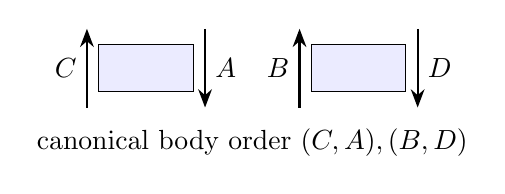
\begin{tikzpicture}[>=Stealth,wire/.style={thick},slot/.style={draw,minimum width=1.2cm,minimum height=.6cm,fill=blue!8}]
  \draw[wire,->] (0,0)--(0,1) node[midway,left] {$C$};
  \draw[wire,->] (1.5,1)--(1.5,0) node[midway,right] {$A$};
  \node[slot] at (.75,.5) {};
  \draw[wire,->] (2.7,0)--(2.7,1) node[midway,left] {$B$};
  \draw[wire,->] (4.2,1)--(4.2,0) node[midway,right] {$D$};
  \node[slot] at (3.45,.5) {};
  \node at (2.1,-.45) {canonical body order $(C,A),(B,D)$};
\end{tikzpicture}
\caption{The canonical two-tooth Choi normal form defining a morphism from the channel type $(A,B)$ to $(C,D)$.}
\label{fig:SDet-body}
\end{figure}

\begin{proposition}[Composition and identities]
Typed composition preserves positivity and the deterministic normalization
equations, is associative, and has the forwarding superchannel as identity.
\end{proposition}
\begin{proof}
This is the two-tooth instance of the deterministic-comb realization and
composition theorem \cite{chiribella2009,chiribella2013}. In the present
components, associativity is associativity of the finite indexed
contraction. The identity on $X=(A,B)$ has Choi operator
\[
R_{\id_X}=J(\id_A)\otimes J(\id_B),
\]
where the first factor is ordered as
$A_{\mathrm{ext}}\otimes A_{\mathrm{src}}$ and the second as
$B_{\mathrm{src}}\otimes B_{\mathrm{ext}}$. The two identity laws follow from the typed link product of
Definition~\ref{def:typed-link}: linking an identity Choi operator to an
open wire gives the same open wire after the declared partial transpose
and canonical orientation permutation. The identity laws are the Choi
snake identities in this fixed convention; their component form is
given in Appendix~\ref{app:category-checks}. The same typed contraction,
applied at each normalization level, proves preservation of the
deterministic equations. Positivity preservation is the standard
composition theorem for deterministic combs with this Choi
ordering, cited above. For a direct normalization check, define the
composite prefix by
\[
H^{(1)}:=\operatorname{Link}_{C}(G^{(1)},F^{(1)}).
\]
Using $\Tr_A F^{(1)}=I_C$ and $\Tr_CG^{(1)}=I_P$ gives
$\Tr_AH^{(1)}=I_P$. Using
$\Tr_D R_F=I_B\otimes F^{(1)}$ and
$\Tr_Q R_G=I_D\otimes G^{(1)}$ in the same typed link gives
$\Tr_QR_{G\circ F}=I_B\otimes H^{(1)}$. Thus the composite satisfies
both deterministic normalization equations.
\end{proof}

\begin{lemma}[Affine hom-sets]
Every hom-set of $\SDet$ is a nonempty compact convex subset of a finite-dimensional real vector space, and composition is affine in each argument.
\end{lemma}
\begin{proof}
The hom-set is the intersection of the positive cone with affine linear
normalization equations, hence is closed and convex. It is nonempty for
arbitrary $(A,B),(C,D)$: choose
\[
R^{(1)}=I_C\otimes\frac{I_A}{d_A},
\qquad
R=I_B\otimes R^{(1)}\otimes\frac{I_D}{d_D},
\]
with the fixed canonical permutation understood. Then
$\Tr_A R^{(1)}=I_C$ and
$\Tr_D R=I_B\otimes R^{(1)}$, and $R$ is positive definite. The fixed
trace of each normalized comb body gives boundedness, hence compactness.
The typed link product is bilinear, and therefore affine in either
argument on the normalized affine sets.
\end{proof}

\begin{remark}[Affine enrichment and dimension polynomial]
The category $\SDet$ is enriched over compact convex sets: its hom-sets are
compact convex sets and composition is affine in each variable. For a fixed
target $Y$, the dimension polynomial
\[
P_Y(u,v):=\affdim\SDet((A,B),Y)
\]
has the form
\[
P_Y(u,v)=\alpha_Yuv+\beta_Yu-\beta_Y
\]
(Proposition~\ref{prop:hom-dim}).
Environment decoration acts by $(u,v)\mapsto(eu,ev)$. The theorem says
that $P_Y(eu,ev)$ is not the dimension polynomial of any representing
object when $e>1$, because the normalization relation between its constant
term and its source-linear coefficient is violated. The obstruction is
affine-dimensional rather than cardinality-based: convex sets of different
finite affine dimensions can have the same cardinality.
\end{remark}

\begin{remark}[Normalization defect]
For a one-slot target $Y$, the normalization defect is the rigid relation
\[
\text{constant term}=-\beta_Y
\]
between the constant term and the source-linear coefficient in
$P_Y(u,v)=\alpha_Yuv+\beta_Yu-\beta_Y$. Environment decoration preserves
the constant term but rescales the source-linear coefficient, which is
the coefficient-rigidity mechanism behind the intercept principle.
\end{remark}

\begin{remark}[Bulk prefactor and normalization defect]
The factor $uv=d_A^2d_B^2$ multiplying $\alpha_Y$ is the full real
ambient dimension of the source channel Choi space. Every later output
fiber is tensored with this source space. The term
$\beta_Yu-\beta_Y$, by contrast, is created by the first preprocessing
tooth and its normalization equation. This separates output bulk from
source normalization. In the auxiliary sequential-body construction,
the corresponding separation is $(1+S)uv-u$; the sequential-body
convention is distinct and does not enter the definition of $\SDet$.
\end{remark}

\section{Environment decoration functor}

Fix a finite-dimensional Hilbert space $E$. For every system occurrence
choose a distinct labeled copy of $E$.

\begin{definition}[Environment decoration on objects]
The object operation is
\[
\Theta_E(A,B):=(A\otimes E,B\otimes E).
\]
Define the object part of the functor by
\[
T_E(X):=\Theta_E(X).
\]
In a displayed morphism, tagged copies of $E$ are used only to record
tensor-factor occurrences; they are not additional object data. When an
object occurs as the target of one morphism and the source of the next,
the tagged copies at matching intermediate tensor positions are identified
by the fixed coherence unitaries before linking.
\end{definition}

\begin{definition}[Environment decoration on morphisms]
Let
\[
R_F\in\SDet((A,B),(C,D)).
\]
Let $J_{E_1E_2}=J(\id_E)$ denote the unnormalized Choi operator of the
identity channel from the first labeled environment occurrence to the
second. Define
\[
T_E(R_F):=\Pi_E\left[
R_F\otimes
J_{E_{C,\mathrm{ext}}E_{A,\mathrm{slot}}}
\otimes
J_{E_{B,\mathrm{slot}}E_{D,\mathrm{ext}}}
\right]\Pi_E^\dagger,
\]
where $\Pi_E$ is the permutation unitary
\[
\begin{aligned}
\Pi_E:
&\bigl(C\otimes A\otimes B\otimes D\bigr)
\otimes\bigl(E_{C,\mathrm{ext}}\otimes E_{A,\mathrm{slot}}\bigr)
\otimes\bigl(E_{B,\mathrm{slot}}\otimes E_{D,\mathrm{ext}}\bigr)\\
&\longrightarrow
(C\otimes E_{C,\mathrm{ext}})\otimes
(A\otimes E_{A,\mathrm{slot}})\otimes
(B\otimes E_{B,\mathrm{slot}})\otimes
(D\otimes E_{D,\mathrm{ext}}).
\end{aligned}
\]
The occurrence labels distinguish external target wires from the source
and slot wires. The definition is given directly on the unique Choi normal
form and requires no choice of circuit representative. The inserted
environment factors are illustrated in Figure~\ref{fig:SDet-TE}.
\end{definition}

\begin{figure}[ht]
\centering
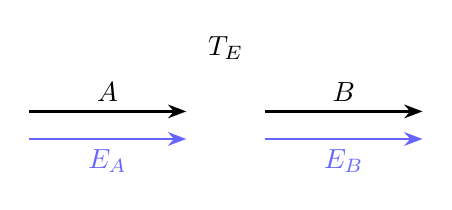
\begin{tikzpicture}[>=Stealth,wire/.style={thick},Ewire/.style={thick,blue!60}]
  \draw[wire,->] (0,0)--(2,0) node[midway,above] {$A$};
  \draw[Ewire,->] (0,-.35)--(2,-.35) node[midway,below,blue!60] {$E_A$};
  \draw[wire,->] (3,0)--(5,0) node[midway,above] {$B$};
  \draw[Ewire,->] (3,-.35)--(5,-.35) node[midway,below,blue!60] {$E_B$};
  \node at (2.5,.8) {$T_E$};
\end{tikzpicture}
\caption{Choi-level environment decoration inserts identity Choi factors on the two body teeth. The environment labels are part of the fixed tensor convention.}
\label{fig:SDet-TE}
\end{figure}

\begin{lemma}[Open identity-wire link]
\label{lem:open-wire}
For isomorphic copies $U,V,W$ of the fixed Hilbert space $E$, put
\[
J_{UV}:=J(\id_{U\to V})\in\Herm(U\otimes V),
\qquad \Tr_VJ_{UV}=I_U.
\]
With the composition order $R_{G\circ F}=\operatorname{Link}(R_G,R_F)$,
the identity-wire law is
\[
J_{VW}*_{V}J_{UV}=J_{UW},
\]
where $*_V$ is the one-wire instance of Definition~\ref{def:typed-link}
with the declared orientation permutation.
\end{lemma}
\begin{proof}
In the fixed Choi bases,
\[
(J_{UV})_{uv,u'v'}=\delta_{uv}\delta_{u'v'},
\qquad
(J_{VW})_{vw,v'w'}=\delta_{vw}\delta_{v'w'}.
\]
Expanding the typed link definition, including its partial transpose and
its declared output orientation, gives the crossed contraction in which
the two intermediate $V$ indices are summed. The resulting entries are
\[
\sum_{v,v'}\delta_{vw}\delta_{v'w'}\delta_{uv}\delta_{u'v'}
=\delta_{uw}\delta_{u'w'},
\]
which are the entries of $J_{UW}$ in the surviving order. No
closed loop is formed, so no factor $d_E$ occurs. The general
identity-wire statement follows by tensoring with unlinked factors.
\end{proof}

\begin{lemma}[Factorization of decorated links]
For composable $F$ and $G$, with matching intermediate environment
occurrences identified, the typed link product satisfies
\[
\operatorname{Link}_{\Theta_E(C,D)}
\bigl(T_E(R_G),T_E(R_F)\bigr)
=
T_E\bigl(\operatorname{Link}_{C,D}(R_G,R_F)\bigr).
\]
Equivalently, up to the declared permutations, the non-environment
factors link as before while the environment factors contract by
\[
J_{E_{P,\mathrm{ext}}E_{C,\mathrm{int}}}
*_{E_{C,\mathrm{int}}}
J_{E_{C,\mathrm{int}}E_{A,\mathrm{slot}}}
=J_{E_{P,\mathrm{ext}}E_{A,\mathrm{slot}}}
\]
and the analogous identity on the $D$ wire.
\end{lemma}
\begin{proof}
Use the same total-space embeddings and partial transpose as
Definition~\ref{def:typed-link}. In the fixed product bases, the partial
transpose on the composite linked system
$(C\otimes E_C)\otimes(D\otimes E_D)$ factorizes into the partial
transposes on $C,D,E_C,E_D$, and the decorated output permutation is the
corresponding extension of the undecorated output permutation. After
expanding matrix entries, the non-environment part of the decorated link
is the contraction
that defines $\operatorname{Link}_{C,D}(R_G,R_F)$. The environment part
factorizes into independent sums. For the $C$ wire, the relevant factor is
\[
\sum_{r,r'}
(J_{E_{P,\mathrm{ext}}E_{C,\mathrm{int}}})_{pr,p'r'}
(J_{E_{C,\mathrm{int}}E_{A,\mathrm{slot}}})_{ra,r'a'}
=(J_{E_{P,\mathrm{ext}}E_{A,\mathrm{slot}}})_{pa,p'a'},
\]
with the index order understood after the orientation permutation in the
link definition. Analogously, the $D$ wire gives
\[
\sum_{s,s'}
(J_{E_{B,\mathrm{slot}}E_{D,\mathrm{int}}})_{bs,b's'}
(J_{E_{D,\mathrm{int}}E_{Q,\mathrm{ext}}})_{sq,s'q'}
=(J_{E_{B,\mathrm{slot}}E_{Q,\mathrm{ext}}})_{bq,b'q'}.
\]
Thus the original contraction and the two independent identity-wire
contractions separate, and the final fixed permutation is the
permutation in the definition of $T_E$. This proves the factorization;
the component form is recorded in Appendix~\ref{app:decorated-factorization}.
\end{proof}

\begin{proposition}[Normalization preservation]
If $R_F\in\SDet((A,B),(C,D))$, then
\[
T_E(R_F)\in\SDet(\Theta_E(A,B),\Theta_E(C,D)).
\]
\end{proposition}
\begin{proof}
By definition of the decorated prefix,
\[
T_E(R_F)^{(1)}=
\frac{1}{d_Bd_E}\Tr_{B E_{B,\mathrm{slot}}D E_{D,\mathrm{ext}}}T_E(R_F).
\]
Since $\Tr_{BD}R_F=d_B R_F^{(1)}$ and
$\Tr_{E_{B,\mathrm{slot}}E_{D,\mathrm{ext}}}
J_{E_{B,\mathrm{slot}}E_{D,\mathrm{ext}}}=d_E$, the factors $d_Bd_E$
cancel and, up to $\Pi_E$,
\[
T_E(R_F)^{(1)}=R_F^{(1)}\otimes J_{E_{C,\mathrm{ext}}E_{A,\mathrm{slot}}}.
\]
Therefore
\[
\Tr_{A E_{A,\mathrm{slot}}}T_E(R_F)^{(1)}
=\Tr_A R_F^{(1)}\otimes\Tr_{E_{A,\mathrm{slot}}}J_{E_{C,\mathrm{ext}}E_{A,\mathrm{slot}}}
=I_C\otimes I_{E_{C,\mathrm{ext}}}
=I_{C\otimes E_{C,\mathrm{ext}}}.
\]
For the second equation,
\[
\Tr_{D E_{D,\mathrm{ext}}}T_E(R_F)
=(\Tr_D R_F)\otimes J_{E_{C,\mathrm{ext}}E_{A,\mathrm{slot}}}\otimes I_{E_{B,\mathrm{slot}}}.
\]
Using $\Tr_D R_F=I_B\otimes R_F^{(1)}$ and reordering gives
\[
\Tr_{D E_{D,\mathrm{ext}}}T_E(R_F)
=I_{B\otimes E_{B,\mathrm{slot}}}\otimes T_E(R_F)^{(1)}.
\]
Positivity is preserved by tensoring and permutation.
\end{proof}

\begin{proposition}[Environment decoration is an affine endofunctor]
\label{prop:TE-strict}
The map $T_E:\SDet\to\SDet$ preserves identities and composition and is linear on the ambient Hermitian Choi spaces. In particular it is affine on every hom-set.
\end{proposition}
\begin{proof}
For $X=(A,B)$, the identity representative has factors ordered as
$J_{A_{\mathrm{ext}}A_{\mathrm{src}}}$ and
$J_{B_{\mathrm{src}}B_{\mathrm{ext}}}$. Applying the definition of $T_E$
adds the factors
\[
J_{E_{A,\mathrm{ext}}E_{A,\mathrm{src}}},
\qquad
J_{E_{B,\mathrm{src}}E_{B,\mathrm{ext}}}.
\]
After the fixed permutation these are the two identity factors
for the enlarged object $T_E(X)$, so
\[
T_E(\id_X)=\id_{T_E(X)}.
\]

For composable $F$ and $G$, the factorization lemma gives
\[
\operatorname{Link}_{\Theta_E(C,D)}
\bigl(T_E(R_G),T_E(R_F)\bigr)
=T_E\bigl(\operatorname{Link}_{C,D}(R_G,R_F)\bigr).
\]
Thus, after the fixed output permutation,
\[
T_E(G)\circ T_E(F)=T_E(G\circ F).
\]
Linearity is immediate from the definition: tensoring with fixed Choi
operators and applying $\Pi_E$ is linear.
\end{proof}

\section{Affine dimensions and coefficient rigidity}

\begin{proposition}[One-slot hom-set dimension]
\label{prop:hom-dim}
For $X=(A,B)$ and $Y=(C,D)$ in $\SDet$,
\[
\affdim\SDet((A,B),(C,D))
=d_C^2(d_A^2-1)+d_C^2d_A^2d_B^2(d_D^2-1).
\]
Putting $u=d_A^2$, $v=d_B^2$,
\[
P_Y(u,v)=\alpha_Yuv+\beta_Yu-\beta_Y,
\]
where
\[
\alpha_Y=d_C^2(d_D^2-1),
\qquad \beta_Y=d_C^2.
\]
\end{proposition}
\begin{proof}
The fixed body order is $(C,A),(B,D)$. The first fiber contributes
$d_C^2(d_A^2-1)$ and the second contributes
$d_C^2d_A^2d_B^2(d_D^2-1)$. The general partial-trace fiber argument is
proved in Appendix~\ref{app:dimension}; the positive-definite point and
fixed-trace compactness argument there show that positivity does not
lower the affine dimension.
\end{proof}

\begin{lemma}[Affine dimension under affine bijection]
If $K$ and $L$ are nonempty convex subsets of finite-dimensional real
vector spaces and there is an affine bijection $K\to L$, then
\[
\affdim K=\affdim L.
\]
\end{lemma}
\begin{proof}
Let $x_0,\ldots,x_r$ be affinely independent in $K$. If their images
were affinely dependent, there would be scalars $\lambda_i$, not all zero,
with $\sum_i\lambda_i=0$ and $\sum_i\lambda_i f(x_i)=0$. Separating the
positive and negative coefficients and normalizing gives equality between
two convex combinations of the images. Affinity of $f$ identifies these
with the images of the corresponding convex combinations in $K$;
injectivity of $f$ then gives equality of those combinations in $K$, a
contradiction. Thus $f$ preserves affine independence. Applying the same
argument to an affinely independent set in $L$ and using surjectivity gives
the reverse inequality, so the affine dimensions agree.
\end{proof}

\begin{lemma}[Polynomial grid]
If a polynomial $q(u,v)$ has degree at most one in each variable and
vanishes for all $u,v\in\{1,4,9,\ldots\}$, then $q$ is the zero polynomial.
\end{lemma}
\begin{proof}
For each fixed allowed $v$, $q(\cdot,v)$ is affine and has infinitely many
zeros, so it is zero. Its two coefficients are affine functions of $v$
that vanish for infinitely many allowed $v$, hence are zero.
\end{proof}

\begin{theorem}[No affine representing object]
For every target object $Y\in\SDet$ and every finite-dimensional
$E$ with $d_E>1$, there is no object $Z\in\SDet$ for which affine
bijections
\[
\SDet(\Theta_EX,Y)\cong\SDet(X,Z)
\]
exist for every source object $X$.
\end{theorem}
\begin{proof}
Write $Y=(C,D)$ and $Z=(C',D')$. Put
\[
u=d_A^2,\qquad v=d_B^2,\qquad e=d_E^2.
\]
The left affine dimension is first obtained by the substitution
$u\mapsto eu$, $v\mapsto ev$:
\[
\affdim\SDet(\Theta_E(A,B),Y)
=d_C^2(eu-1)+d_C^2(eu)(ev)(d_D^2-1).
\]
Thus it is
\[
e^2\alpha_Yuv+e\beta_Yu-\beta_Y,
\qquad
\alpha_Y=d_C^2(d_D^2-1),\quad \beta_Y=d_C^2,
\]
whereas the right dimension is
\[
\alpha_Zuv+\beta_Zu-\beta_Z,
\qquad \beta_Z=d_{C'}^2>0.
\]
By the affine-dimension lemma, each affine bijection gives equality of
affine dimensions. By the polynomial-grid lemma, equality on the infinite
squared-dimension grid forces equality as polynomials in $u,v$. Comparing
the three monomials gives
\[
\alpha_Z=e^2\alpha_Y,
\qquad
\beta_Z=e\beta_Y,
\qquad
\beta_Z=\beta_Y.
\]
Since $\beta_Y>0$, $e=1$, contradicting $d_E>1$.
\end{proof}

\begin{remark}[Trivial environment]
When $d_E=1$, the object operation $\Theta_E$ is canonically isomorphic to
the identity object operation, and the identity functor provides a right
adjoint in this case; being self-adjoint, it is likewise a left adjoint.
\end{remark}

\begin{proposition}[Affine transposition in affine-enriched categories]
Let $\mathcal C$ be a category whose hom-sets are convex sets and whose
composition is affine in each variable. Let $H:\mathcal C\to\mathcal C$ be
an affine endofunctor. If $H$ has a right adjoint $G$, every adjunction
bijection
\[
\mathcal C(HX,Y)\cong\mathcal C(X,GY)
\]
is affine. Both $\SDet$ and $\mathbf{Chan}$ satisfy these hypotheses.
\end{proposition}
\begin{proof}
The inverse transposition sends $g:X\to GY$ to
$\varepsilon_Y\circ H(g)$. Since $H$ is affine and composition is affine
in each variable, this inverse transposition is affine. A bijective affine
map between convex sets has an affine inverse by the elementary
convex-combination argument in Appendix~\ref{app:affinity}.
\end{proof}

\begin{theorem}[No right adjoint for environment decoration]
Let $E$ be finite-dimensional with $d_E>1$. Since $T_E$ is an affine endofunctor by Proposition~\ref{prop:TE-strict}, the affine nonrepresentability theorem implies that the affine endofunctor
\[
T_E:\SDet\to\SDet
\]
has no right adjoint.
\end{theorem}
\begin{proof}
If $T_E\dashv G$, Proposition~\ref{prop:TE-strict} and the affine
transposition lemma give affine bijections
\[
\SDet(T_EX,Y)\cong\SDet(X,GY)
\]
for every $X,Y$. Since $T_EX=\Theta_E X$, this contradicts the no-affine-
representing-object theorem with $Z=GY$.
\end{proof}

\begin{corollary}[Any affine extension has no right adjoint]
Let $F:\SDet\to\SDet$ be an affine endofunctor whose object map is
$F(X)=\Theta_E(X)$ up to the fixed coherence isomorphisms. If $d_E>1$,
then $F$ has no right adjoint.
\end{corollary}
\begin{proof}
If $F\dashv G$, the generalized affine-transposition proposition gives
affine bijections
\[
\SDet(FX,Y)\cong\SDet(X,GY).
\]
The coherence isomorphism $F(X)\cong\Theta_E(X)$ induces, by precomposition,
an affine isomorphism
\[
\SDet(FX,Y)\cong\SDet(\Theta_E X,Y).
\]
Composing these bijections gives affine representing bijections of the
type ruled out by the no-affine-representing-object theorem. Hence no
right adjoint exists.
\end{proof}

\begin{example}[Qubit source and target]
Take $X=Y=(\mathbb C^2,\mathbb C^2)$ and $E=\mathbb C^2$. Then
$u=v=e=4$, $\alpha_Y=12$, and $\beta_Y=4$. The unextended hom-set
has affine dimension
\[
4(4-1)+4\cdot4\cdot4\cdot3=204,
\]
whereas the decorated hom-set has dimension
\[
4(16-1)+4\cdot16\cdot16\cdot3=3132.
\]
Writing the candidate representing object as $Z=(C',D')$, the
polynomial comparison gives $\beta_Z=4$ from the constant term and
$\beta_Z=16$ from the coefficient of $u$, which already excludes
representability. Independently, evaluation of the dimension polynomials
at $u=v=4$ gives
\[
3132=16\alpha_Z+3\beta_Z,
\]
hence $\alpha_Z=195$. Since in the one-slot category
$\alpha_Z=\beta_Z(d_{D'}^2-1)=4(d_{D'}^2-1)$, the single-point evaluation
confirms the same obstruction.
\end{example}

\begin{proposition}[Affine transposition for left adjoints]
Let $\mathcal C$ be a category whose hom-sets are convex sets and whose
composition is affine in each variable. Let $K:\mathcal C\to\mathcal C$
be an affine endofunctor. If $K$ has a left adjoint $L$, every adjunction
bijection
\[
\mathcal C(LY,X)\cong\mathcal C(Y,KX)
\]
is affine.
\end{proposition}
\begin{proof}
The forward transposition sends $f:LY\to X$ to
$K(f)\circ\eta_Y$, where $\eta:\id\Rightarrow KL$ is the unit. Since
$K$ is affine and composition is affine in each variable, this composite
is affine. A bijective affine map between convex sets has an affine
inverse by the elementary argument of Appendix~\ref{app:affinity}.
\end{proof}

\begin{theorem}[No left adjoint for environment decoration]
Let $E$ be finite-dimensional with $d_E>1$. Then the affine endofunctor
\[
T_E:\SDet\to\SDet
\]
has no left adjoint.
\end{theorem}
\begin{proof}
Put $I=(\mathbb C,\mathbb C)$ and suppose $L\dashv T_E$. By the
left-adjoint affine-transposition proposition, the adjunction bijection
\[
\SDet(LI,I)\cong\SDet(I,T_EI)
\]
is affine, so the two sides have equal affine dimension. Write
$L(I)=(P,Q)$ and set $p=d_P^2$ and $e=d_E^2$.
Proposition~\ref{prop:hom-dim} gives
\[
\affdim\SDet(LI,I)=p-1,
\qquad
\affdim\SDet(I,T_EI)=\affdim\SDet\bigl(I,(E,E)\bigr)=e(e-1).
\]
Equality forces
\[
p=e^2-e+1.
\]
Since $e>1$,
\[
(e-1)^2<e^2-e+1<e^2,
\]
so $p$ lies strictly between consecutive squares and cannot equal
$d_P^2$, a contradiction.
\end{proof}

\begin{corollary}[Any affine extension has no left adjoint]
Let $F:\SDet\to\SDet$ be an affine endofunctor whose object map is
$F(X)=\Theta_E(X)$ up to the fixed coherence isomorphisms. If $d_E>1$,
then $F$ has no left adjoint.
\end{corollary}
\begin{proof}
If $L\dashv F$, the left-adjoint transposition gives an affine bijection
$\SDet(LI,I)\cong\SDet(I,FI)$. Postcomposition with the coherence
isomorphism $F(I)\cong\Theta_E(I)$ is an affine isomorphism of the
target hom-sets, so $\affdim\SDet(I,FI)=\affdim\SDet(I,\Theta_E I)$,
and the computation of the no-left-adjoint theorem applies verbatim.
\end{proof}

\section{Connections and special cases}

\subsection{Toy model: deterministic channels}

The same affine-representability mechanism appears in the ordinary
category $\mathbf{Chan}$ of nonzero finite-dimensional deterministic
channels. For finite-dimensional $A,B$,
\[
\affdim\mathbf{Chan}(A,B)=d_A^2(d_B^2-1),
\]
because a channel Choi operator has real dimension $d_A^2d_B^2$ and the
trace-preserving equation imposes $d_A^2$ independent affine constraints.
Define $\Theta_E^{\mathrm{ch}}(A)=A\otimes E$ on objects and
$\Theta_E^{\mathrm{ch}}(\Phi)=\Phi\otimes\id_E$ on channels. This is an
affine endofunctor of $\mathbf{Chan}$.

If it had a right adjoint $G$, affine transposition would force, for fixed
$B$ and all $A$,
\[
\affdim\mathbf{Chan}(A\otimes E,B)
=\affdim\mathbf{Chan}(A,GB).
\]
Writing $u=d_A^2$, $e=d_E^2$, and $g_B=d_{GB}^2$, this gives
\[
eu(d_B^2-1)=u(g_B-1),
\qquad g_B=e(d_B^2-1)+1.
\]
Taking $B=E$ yields
\[
g_E=e^2-e+1.
\]
For $e>1$,
\[
(e-1)^2<e^2-e+1<e^2,
\]
so $g_E$ lies strictly between consecutive squares and cannot equal
$d_{GE}^2$. Thus channel environment decoration has no right adjoint
when $d_E>1$. The obstruction here is of perfect-square type, distinct
from the coefficient-rigidity obstruction in $\SDet$; the channel model
is self-contained and is not used in the superchannel theorem.

\subsection{Toy model: finite classical stochastic maps}

The same obstruction structure appears at the classical level. Let
$\mathbf{FinStoch}$ be the category of nonempty finite sets and
stochastic kernels $f(b\mid a)$. Its hom-sets are convex polytopes and
composition is matrix multiplication, hence affine in each variable. For
a finite environment set $E$ with $|E|=e>1$, define
\[
\Theta_E^{\mathrm{cl}}(A)=A\times E,
\qquad
\Theta_E^{\mathrm{cl}}(f)(b,e'\mid a,e)=f(b\mid a)\,\delta_{e',e},
\]
an affine endofunctor of $\mathbf{FinStoch}$.

\begin{proposition}[Classical environment decoration has neither adjoint]
For $|E|=e>1$, the functor
$\Theta_E^{\mathrm{cl}}:\mathbf{FinStoch}\to\mathbf{FinStoch}$ has no
right adjoint and no left adjoint.
\end{proposition}
\begin{proof}
Suppose $G$ were a right adjoint. The affine-transposition hypotheses
hold for $\mathbf{FinStoch}$, so the adjunction bijection
$\mathbf{FinStoch}(A\times E,B)\cong\mathbf{FinStoch}(A,GB)$ is affine.
This bijection and its inverse are affine, so both the affine dimension
and the number of extreme points are preserved. Take
$A$ a singleton and $|B|=b>1$. The left hom-set is the product of $e$
copies of the simplex $\Delta_{b-1}$ of probability vectors on $b$
points, of affine dimension $e(b-1)$ with $b^e$ vertices. The right
hom-set is the single simplex $\Delta_{g-1}$ on $g=|GB|$ points, of
dimension $g-1$ with $g$ vertices. Hence
\[
g-1=e(b-1),
\qquad
g=b^e,
\]
so $b^e-1=e(b-1)$. For $b,e>1$,
\[
b^e-1=(b-1)\sum_{k=0}^{e-1}b^k>e(b-1),
\]
since the sum has $e$ terms, each at least $1$, and all but the $k=0$
term at least $2$; a contradiction.

Suppose instead $L\dashv\Theta_E^{\mathrm{cl}}$. The left-adjoint
transposition gives an affine bijection
$\mathbf{FinStoch}(LY,X)\cong\mathbf{FinStoch}(Y,X\times E)$. With
$Y=X$ a singleton, the left side is a single point, of affine dimension
$0$, whereas the right side is the simplex of probability vectors on
$E$, of dimension $e-1>0$; a contradiction.
\end{proof}

The classical right-adjoint obstruction is a vertex-count obstruction,
rather than the coefficient rigidity used in $\SDet$, and the classical
left-adjoint obstruction is the singleton-versus-simplex mismatch; the
normalization term $-|A|$ of Table~\ref{tab:comparative} is their
affine-dimension counterpart.

\subsection{Instruments and the pointwise obstruction}

An $n$-outcome instrument from $A$ to $B$ is described by $n$ positive Choi
operators whose sum is trace-preserving, giving the affine dimension
\[
nd_A^2d_B^2-d_A^2=d_A^2(nd_B^2-1).
\]
This comparison is illustrative and does not by itself constitute a formal
adjunction result. A categorical treatment would require defining
instrument objects, morphisms, outcome-count composition, and environment
decoration. A pointwise obstruction at fixed outcome number is proved in
Appendix~\ref{app:instr} and is included as the instrument row of
Table~\ref{tab:comparative}; no instrument result is used in the main
theorem.

\subsection{CP maps and the normalized subcategory}

The obstruction is not caused by complete positivity alone. The CPM construction associated with finite-dimensional Hilbert spaces is dagger compact closed, so unrestricted completely positive maps admit the corresponding compact-closed currying structure \cite{selinger2007,coeckekissinger2017}. Explicitly, tensoring with the environment has there the right adjoint $E^*\otimes-$,
\[
\mathbf{CPM}(A\otimes E,B)\cong\mathbf{CPM}(A,E^*\otimes B),
\]
and the transpose of a trace-preserving map under this bijection need not be trace-preserving. The trace-preserving one-slot category $\SDet$ is a normalized subcategory. The compact-closed construction need not preserve its trace-preserving equations, and the coefficient rigidity proved above is the affine-dimensional manifestation of that failure.

\subsection{Quantum error correction and Petz recovery}

At morphism level, exact quantum error correction is governed by conditions such as the Knill--Laflamme equations. If $P$ projects onto a code space and $\{K_k\}$ are Kraus operators, exact correctability is equivalent to
\[
 P K_k^\dagger K_\ell P=\alpha_{k\ell}P
\qquad\text{for all }k,\ell.
\]
Equivalently, the complementary channel is constant on the code space. Under suitable support assumptions, a Petz recovery map can recover the code states from the noisy output \cite{petz1986,knilllaflamme1997,hayden2004}.

The Petz map associated with a reference state $\sigma$ and channel $\Phi$ is
\[
\mathcal R_{\sigma,\Phi}(X)
=
\sigma^{1/2}\Phi^*\!\left(
\Phi(\sigma)^{-1/2}X\Phi(\sigma)^{-1/2}
\right)\sigma^{1/2},
\]
where $\Phi^*$ denotes the Hilbert--Schmidt adjoint of $\Phi$, and the inverse is taken on the support of $\Phi(\sigma)$, or equivalently interpreted as a generalized inverse. When the relevant sufficiency conditions hold, this map recovers the states in the code sector. If a globally trace-preserving channel on the full output algebra is required, the supported recovery map must be completed by an arbitrary CPTP extension on the orthogonal complement; that extension is not unique and is irrelevant to the code-sector statement.

For completeness, the two levels can be displayed explicitly:
\begin{itemize}
\item \textbf{Morphism level.} An individual channel or comb may have a left inverse on a code subspace, or may admit a state-dependent recovery map. The corresponding complementary process then carries no relevant input-dependent information on that code.
\item \textbf{Functorial level.} A right adjoint would assign a representing recovery object to every output interface and would induce affine bijections for every source interface simultaneously. The theorem rules out this universal assignment even before naturality is imposed.
\end{itemize}

These are morphism-level statements, whereas the main theorem is functorial: it says that there is no single right-adjoint assignment providing a universal representing recovery process for all objects of $\SDet$. An individual comb can therefore be recoverable even though $T_E$ has no right adjoint in $\SDet$. The two failures are logically independent.

The higher-order analogue of the Knill--Laflamme condition would require a complementary comb to be constant on the relevant family of input combs. Developing that condition is a separate problem and is not needed for the present no-representing-object theorem.

This distinction also differs from the no-cloning theorem \cite{dieks1982,wootters1982}. No-cloning concerns a universal operation on unknown states, whereas the present result concerns universal currying of an environment in a fixed-order normalized process category. Both reflect the non-Cartesian structure of quantum theory, in which the monoidal product is not a categorical product; they differ in the level of the process hierarchy at which the universal operation is demanded.

\subsection{Arbitrary order and left adjoints}

The theorem is proved for the one-slot category $\SDet$. The extension to the full deterministic process hierarchy is established in Appendix~\ref{app:allorders}, which supplies the canonical multi-slot Choi normal form and the composition theorem: the objects are comb types of arbitrary finite arity, the morphisms are deterministic combs in the interleaved wire normal form, composition is the link product, and the hom-set affine dimension is the telescoping polynomial $\sum_t\bigl(\prod_{i<2t}w_i\bigr)(w_{2t}-1)$ in the squared wire dimensions. The right-adjoint obstruction at every arity is the same rigidity pair as in Section 4, with the constant term equal to the negative of the coefficient of the first source variable; the left-adjoint obstruction at every arity is a comparison of the maximal target monomial between target arities one and two and requires no arithmetic between consecutive squares. Environment decoration therefore has neither adjoint at any finite order of the hierarchy.

The left-adjoint question is settled in the negative in Section 4, and its tester mechanism is visible directly. By the normalization equations, a morphism $(A,B)\to(\mathbb C,\mathbb C)$ has Choi operator $I_B\otimes\rho$ with $\rho$ a density operator on $A$, and such tester-type morphisms satisfy
\[
\affdim\SDet\bigl((A,B),(\mathbb C,\mathbb C)\bigr)=d_A^2-1.
\]
That theorem is proved by evaluating at this trivial object: adjointability with source $L(I)=(P,Q)$ would force $d_P^2=e^2-e+1$, strictly between consecutive squares. The hom-set into $(\mathbb C,\mathbb C)$ is high-dimensional whenever $d_A>1$; in particular, $(\mathbb C,\mathbb C)$ is not a terminal object of $\SDet$. Abstract left-adjoint arguments based on terminality therefore do not apply; the obstruction is the tester dimension itself.

\subsection{Summary of mechanisms and notation}

Table~\ref{tab:mechanisms} places the two normalization mechanisms used
in this paper side by side: the standard-superchannel mechanism that
supports the main theorem, and the auxiliary sequential-body mechanism.
Table~\ref{tab:comparative} collects the affine-dimension mechanisms
across the channel, instrument, comb, and classical settings, together
with the status of each row. Table~\ref{tab:notation} summarizes the
recurring notation.

\begin{table}[ht]
\centering
\begin{tabular}{lll}
\toprule
Construction & Dimension form & Environment effect\\
\midrule
Standard superchannel & $\alpha uv+\beta u-\beta$ & $(\alpha,\beta,-\beta)\mapsto(e^2\alpha,e\beta,-\beta)$\\
Sequential body & $(1+S)uv-u$ & $(1+S,-1)\mapsto(e^2(1+S),-e)$\\
\bottomrule
\end{tabular}
\caption{The two normalization mechanisms used in the paper. The sequential-body row is auxiliary; the standard-superchannel row supports the categorical theorem.}
\label{tab:mechanisms}
\end{table}

\begin{table}[ht]
\centering
\begin{tabular}{llll}
\toprule
Category & Hom-set dimension & Normalization term & Status\\
\midrule
$\mathbf{Chan}$ & $d_A^2(d_B^2-1)$ & $-d_A^2$ & Proved toy model\\
$\mathbf{Instr}_n$ & $d_A^2(nd_B^2-1)$ & $-d_A^2$ & Pointwise result (App.~\ref{app:instr})\\
Standard $\SDet$ & $\alpha uv+\beta u-\beta$ & $-\beta$ & Proved here\\
Sequential body & $(1+S)uv-u$ & $-u$ & Auxiliary appendix\\
$\mathbf{FinStoch}$ & $|A|(|B|-1)$ & $-|A|$ & Proved toy model\\
\bottomrule
\end{tabular}
\caption{Dimension mechanisms across normalized process settings. Only the standard-comb row is used for the main theorem. The channel and $\mathbf{FinStoch}$ rows are proved toy models, the instrument row is a pointwise result proved in Appendix~\ref{app:instr}, and the sequential-body row is auxiliary.}
\label{tab:comparative}
\end{table}

\begin{table}[ht]
\centering
\begin{tabular}{ll}
\toprule
Symbol & Meaning\\
\midrule
$d_X$ & Dimension of the Hilbert space $X$\\
$u,v$ & $d_A^2,d_B^2$ for the source channel\\
$S$ & Sequential-body sum of the auxiliary construction\\
$e$ & $d_E^2$ for the environment\\
$\alpha_Y$ & Bulk coefficient for a target object\\
$\beta_Y$ & First-target-input squared dimension\\
$\Theta_E$ & Environment-decoration object operation\\
$\Theta_E^{\mathrm{ch}}$ & Channel environment-decoration operation\\
$T_E$ & Environment-decoration endofunctor\\
$G$ & Hypothetical right adjoint\\
$L$ & Hypothetical left adjoint\\
\bottomrule
\end{tabular}
\caption{Notation summary.}
\label{tab:notation}
\end{table}

\section{Parallel tensor product and closedness}

The canonical parallel tensor product on $\SDet$ is defined directly from
the Choi representatives. On objects, put
\[
(A,B)\otimes(C,D)=(A\otimes C,B\otimes D),
\qquad
I_\otimes=(\mathbb C,\mathbb C),
\]
and on morphisms $F:X\to Y$ and $G:P\to Z$, let $F\otimes G$ be the
morphism with Choi operator $R_F\otimes R_G$ and prefix
$R_F^{(1)}\otimes R_G^{(1)}$, regarded in the fixed tensor convention
after the canonical permutations.

\begin{lemma}[Parallel tensor is a monoidal product]
\label{lem:parallel}
The parallel tensor is a well-defined bifunctor
$\SDet\times\SDet\to\SDet$: it preserves positivity and the
deterministic normalization equations, composition, and identities, and
it is affine in each variable. With the strictified tensor convention it
is a strict monoidal product with unit $I_\otimes$.
\end{lemma}
\begin{proof}
For $F:(A,B)\to(C,D)$ and $G:(P,Q)\to(R,S)$, normalization of the
product follows by tracing the disjoint factor sets:
\[
\Tr_{A\otimes P}\bigl(R_F^{(1)}\otimes R_G^{(1)}\bigr)
=I_C\otimes I_R
=I_{C\otimes R},
\]
and
\[
\Tr_{D\otimes S}(R_F\otimes R_G)
=\bigl(I_B\otimes R_F^{(1)}\bigr)\otimes\bigl(I_Q\otimes R_G^{(1)}\bigr)
=I_{B\otimes Q}\otimes\bigl(R_F^{(1)}\otimes R_G^{(1)}\bigr).
\]
Positivity is preserved by tensor product. The interchange law is the
factorization of the typed link product over two disjoint pairs of
linked systems; its component form, with the second factor general
rather than an identity wire, is recorded in
Appendix~\ref{app:decorated-factorization}. Identities and
associativity follow from the strictified convention. Affinity is
bilinearity of the tensor product on the ambient Choi spaces.
\end{proof}

Tensoring by an environment object reproduces environment decoration:
on objects,
\[
X\otimes(E,E)=\Theta_E(X),
\]
and on morphisms, $F\otimes\id_{(E,E)}$ inserts precisely the identity
Choi factors
$J_{E_{C,\mathrm{ext}}E_{A,\mathrm{slot}}}\otimes
J_{E_{B,\mathrm{slot}}E_{D,\mathrm{ext}}}$
of the decoration map. Hence $-\otimes(E,E)$ is an affine endofunctor
whose object part is $\Theta_E$ up to the fixed coherence isomorphisms.

\begin{corollary}[The parallel tensor product is not closed]
\label{cor:not-closed}
If $d_E>1$, the endofunctor $-\otimes(E,E):\SDet\to\SDet$ has neither a
right adjoint nor a left adjoint. In particular, the monoidal category
$(\SDet,\otimes,I_\otimes)$ defined above is not right-closed and not
left-closed at any nontrivial environment object.
\end{corollary}
\begin{proof}
A right adjoint contradicts the extension corollary for right adjoints,
and a left adjoint contradicts the extension corollary for left
adjoints.
\end{proof}

\section{Scope}

The scope of the mathematical conclusions is delimited as follows.

\begin{enumerate}
\item The theorems concern right- and left-adjoint representability and do not prove that individual combs are noninvertible.
\item The affine dimension count gives no operational lower bound in trace norm, diamond norm, fidelity, or any other distance.
\item No thermodynamic arrow follows formally. Additional physical assumptions about dynamics, coarse-graining, and boundary conditions would be required \cite{price1996,wallace2023}.
\item The theorem is specific to finite-dimensional, trace-preserving, fixed-order deterministic combs.
\item Monoidal closedness is settled only for the canonical parallel tensor product defined in Section 6, which is not closed at nontrivial environment objects; arbitrary other monoidal structures on $\SDet$ are outside the present scope.
\item Indefinite causal order and process-matrix generalizations require separate definitions and proofs.
\item The positive content is that normalization imposes a coefficient relation on the affine dimension. Environment decoration changes the source-dependent coefficient while leaving the scalar normalization term fixed, so a representing object cannot satisfy the same relation. Mechanically, the first tooth contributes the ambient dimension $\beta_Yu$ of $\Herm(C\otimes A)$ minus the $\beta_Y$ independent scalar equations of $\Tr_A R^{(1)}=I_C$, leaving $\beta_Yu-\beta_Y$; constraint and defect are the same count. Decoration enlarges the traced-out source tooth to $A\otimes E$, so the same $\beta_Y$ equations subtract from an ambient dimension enlarged by the factor $e$, while the equation $\Tr_{A\otimes E}R^{(1)}=I_C$ is a joint constraint that does not split into separate constraints on $A$ and on $E$. A representing object on the undecorated systems has the constraint count and the ambient dimension of the undecorated tooth and cannot reproduce the rescaled relation. The same mechanism structure appears classically in $\mathbf{FinStoch}$ (Table~\ref{tab:comparative}), with stochasticity in place of trace preservation.
\end{enumerate}

The theorems are a categorical obstruction to an adjoint representation, right or left, of the explicitly defined environment-decoration functor on the one-slot category $\SDet$. It does not assert that every individual process with an environment is unrecoverable, nor does it exclude state-dependent Petz recovery, code-subspace error correction, approximate recovery, or special morphism-level splittings. The extension of both statements to the full hierarchy of comb types of arbitrary finite order, built on a canonical interleaved Choi normal form and its composition theorem, is established in Appendix~\ref{app:allorders}; the scope delimitations of that extension are stated there.

The obstruction is a consequence of normalized trace constraints. In the unrestricted CPM setting, the CPM construction is dagger compact closed, so the normalized obstruction is absent at that level \cite{selinger2007}.

\section{Conclusion}

The main theorem establishes a categorical obstruction to universal
environmental currying in the finite-dimensional one-slot deterministic
superchannel category $\SDet$. The result rests on a coefficient relation
forced by normalization. For objects $X=(A,B)$ and $Y=(C,D)$, the standard two-tooth
normal form gives
\[
P_Y(u,v)=\alpha_Yuv+\beta_Yu-\beta_Y.
\]
The coefficient of $u$ and the scalar constant are therefore not
independent. Environment decoration sends
\[
(u,v)\longmapsto(eu,ev),\qquad e=d_E^2,
\]
and hence
\[
P_Y^{\Theta_E}(u,v)=e^2\alpha_Yuv+e\beta_Yu-\beta_Y.
\]
A representing object would have to reproduce both the unchanged
constant term and the rescaled $u$ coefficient. Since its normalization relation is again
\[
\text{constant term}=-\beta,
\]
this is impossible for $e>1$.

The dual obstruction excludes a left adjoint by a separate arithmetic.
At the trivial object $I=(\mathbb C,\mathbb C)$, the morphisms into $I$
are of tester type, with Choi operators $I_B\otimes\rho$ having affine
dimension $d_A^2-1$, while
\[
\affdim\SDet\bigl(I,(E,E)\bigr)=e(e-1).
\]
Affine adjunction at $I$ would therefore force $d_P^2=e^2-e+1$ for the
putative representing object $(P,Q)$, strictly between consecutive
squares for $e>1$. Hence environment decoration has neither a right nor
a left adjoint for a nontrivial environment.

The obstruction is not confined to the one-slot category.
Appendix~\ref{app:allorders} constructs the category of comb types of
arbitrary finite order and proves, by coefficient comparisons in the
telescoping hom-set dimension polynomial, that environment decoration
has neither adjoint at any order. The arity-one instances recover the
statements above; the between-squares arithmetic is needed only at
arity one, while in the full hierarchy the left-adjoint obstruction
already follows from a comparison of target arities one and two.

The theorem is stronger than a statement about a single process. It
rules out even a pointwise assignment of representing objects admitting
affine bijections on all one-slot sources, without requiring naturality.
It does not rule out recovery for particular processes, code subspaces,
or reference states. The two levels differ: functorial adjointability is obstructed by
the global normalization geometry, while morphism-level splitting may hold for
special channels or combs.

The auxiliary sequential-body construction exhibits a related but
different coefficient mechanism. Its dimension polynomial is
\[
(1+S(\mathbf C))uv-u,
\]
and the $v$-intercept changes under environment decoration. This
construction plays no role in the main theorem.

The obstruction is specific to normalized finite-dimensional
fixed-order processes. It is not an operational error bound, a theorem
that every open process is physically unrecoverable, or a derivation of
the thermodynamic arrow. Monoidal closedness is determined only for the
canonical parallel tensor product, which fails at nontrivial environment
objects; other monoidal structures are not treated. What it establishes
is that probability-preserving higher-order structure does not support a
universal adjoint currying operation for a nontrivial external
environment, on either side.

\paragraph{Future directions.}
Natural extensions include trace-nonincreasing and probabilistic
variants, approximate adjunctions, and indefinite-causal-order process
categories. Each extension requires its own typed normal form and
composition theorem.

\appendix

\section{Auxiliary concatenated-body construction}
\label{app:seqbody}

This appendix records an auxiliary dimension calculation for a sequential-body convention, distinct from the hom-set formula of the main text. Define the sequential normalized-body space
\[
\mathsf{SeqDet}(L;\mathbf C):=\Det(((A,B))\concat\mathbf C),
\]
where the concatenation denotes an ordered body sequence. The space
$\mathsf{SeqDet}$ is not identified with the comb space
$\Comb(L,\mathbf C)$; no categorical composition or adjunction is
associated with this construction.

For $\mathbf C=((C_1,D_1),\ldots,(C_n,D_n))$, put
\[
S(\mathbf C)=\sum_{j=1}^n
\left(\prod_{i<j}d_{C_i}^2d_{D_i}^2\right)d_{C_j}^2(d_{D_j}^2-1).
\]
The general deterministic-comb dimension polynomial gives
\[
\affdim\mathsf{SeqDet}(L;\mathbf C)
=d_A^2(d_B^2-1)+d_A^2d_B^2S(\mathbf C).
\]
Writing $u=d_A^2$ and $v=d_B^2$ yields
\[
Q_{\mathbf C}(u,v)=(1+S(\mathbf C))uv-u.
\]
Under source environment decoration, $(u,v)\mapsto(eu,ev)$, so
\[
Q_{\mathbf C}(u,v)\mapsto e^2(1+S(\mathbf C))uv-eu.
\]
Thus, at fixed $u$, the affine intercept as a function of $v$ is scaled from $-u$ to $-eu$ within this auxiliary construction; the geometry is displayed in Figure~\ref{fig:intercept}.

\begin{figure}[ht]
\centering
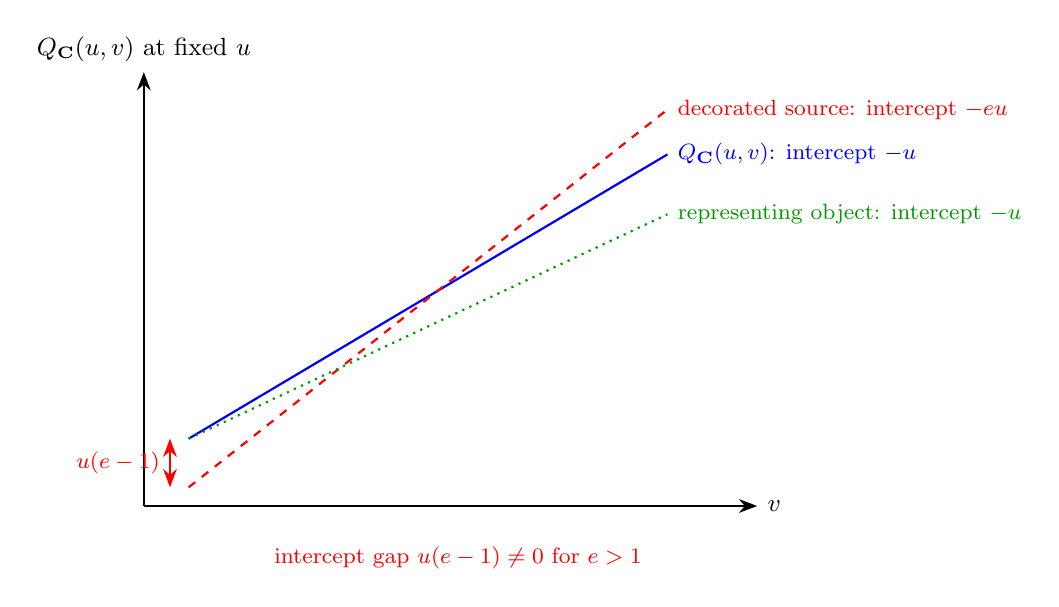
\begin{tikzpicture}[>=Stealth,scale=0.95]
  \draw[->,thick] (0,0) -- (8.2,0) node[right,font=\small] {$v$};
  \draw[->,thick] (0,0) -- (0,5.8) node[above,font=\small] {$Q_{\mathbf C}(u,v)$ at fixed $u$};
  \draw[thick,blue] (0.6,0.9) -- (7,4.7)
    node[right,font=\footnotesize,blue] {$Q_{\mathbf C}(u,v)$: intercept $-u$};
  \draw[thick,red,dashed] (0.6,0.25) -- (7,5.3)
    node[right,font=\footnotesize,red] {decorated source: intercept $-eu$};
  \draw[thick,green!60!black,dotted] (0.6,0.9) -- (7,3.9)
    node[right,font=\footnotesize,green!60!black] {representing object: intercept $-u$};
  \draw[<->,thick,red] (0.35,0.25) -- (0.35,0.9)
    node[midway,left,font=\footnotesize,red] {$u(e-1)$};
  \node[font=\footnotesize,red,align=center] at (4.2,-0.7)
    {intercept gap $u(e-1)\neq0$ for $e>1$};
\end{tikzpicture}
\caption{Schematic of the auxiliary sequential-body mechanism. At fixed $u$, the affine dimension $Q_{\mathbf C}(u,v)=(1+S)uv-u$ is affine in $v$ with intercept $-u$; source decoration multiplies the slope by $e^2$ and gives intercept $-eu$, while every candidate representing object has intercept $-u$ again. The intercept gap $u(e-1)$ is the obstruction within this auxiliary construction.}
\label{fig:intercept}
\end{figure}

\begin{proposition}[Sequential-body obstruction; auxiliary]
Fix a sequential body $\mathbf C$ and let $e=d_E^2>1$. There is no
sequential body $\mathbf C'$ such that
\[
Q_{\mathbf C'}(u,v)=Q_{\mathbf C}(eu,ev)
\quad\text{for all allowed }u,v.
\]
\end{proposition}
\begin{proof}
An undecorated sequential-body polynomial has the form
$Q_{\mathbf C'}(u,v)=(1+S(\mathbf C'))uv-u$, whereas
$Q_{\mathbf C}(eu,ev)=e^2(1+S(\mathbf C))uv-eu$. On the infinite
squared-dimension grid, the polynomial-grid lemma of Section~4 reduces
polynomial equality to coefficient equality, and the source-linear
coefficients give $-1=-e$, hence $e=1$.
\end{proof}

The positive recursive base point used in this calculation is
\[
R^{(1)}=I_A\otimes\frac{I_B}{d_B},
\]
which satisfies
\[
\Tr_B R^{(1)}=I_A.
\]
The same construction proves nonemptiness at every subsequent comb level.

\section{Causal placements and link products}
\label{app:placements}

The standard placement for a channel $A\to B$ inserted into the first tooth of an output comb is
\[
(C_1,A),\quad(B,D_1),\quad(C_2,D_2),\ldots,(C_n,D_n).
\]
It permits arbitrary preprocessing of the external $C_1$ input and arbitrary postprocessing after the unknown channel. It contains the identity superchannel.

The gap-first placement
\[
(\mathbf I,A),\quad(B\otimes C_1,D_1),\ldots
\]
is a restricted tester-like architecture. It does not contain the identity superchannel because the unknown channel cannot receive the arbitrary external $C_1$ input. Later insertion positions define other typed process classes and require separate analyses.

For linked Choi operators we use the typed link product of
Definition~\ref{def:typed-link}. Thus all embeddings, partial transposes,
canonical permutations, and unlinked identity factors are those fixed in
Section~2. In particular, if $X$ and $Y$ are the two Choi operators in an
open environment-wire contraction, the contraction is performed with the
same partial transpose and orientation convention as in the main
composition law. The identity channel satisfies
\[
\Tr_YJ(\id_X)=I_X.
\]
For open environment wires, the typed identity-wire lemma gives the
corresponding surviving identity Choi operator. A completely closed
cup-cap loop can produce a dimension scalar under the unnormalized
convention; no such loop arises in the definition of $T_E$.

\section{Derivation of the typed component link}
\label{app:component-link}

We record the index calculation underlying Definition~\ref{def:typed-link}.
The operators $R_F$ and $R_G$ initially have orders
\[
C,A,B,D\quad\text{and}\quad P,C,D,Q,
\]
respectively. The permutation $U_F$ produces the order $C,D,A,B$, while
$U_G$ produces $P,Q,C,D$. Embedding these into
\[
P,Q,C,D,A,B
\]
produces $\widehat R_F$ and $\widehat R_G$. The partial transpose on the
linked factors exchanges the two matrix indices associated with $C,D$ in
$\widehat R_G$. Taking the partial trace identifies the matching linked
indices and leaves $P,A,B,Q$. The final $U_{\mathrm{out}}$ restores the
declared output order $P,A,B,Q$.

With the orientation convention fixed by these permutations, the resulting
entries are
\[
(R_{G\circ F})_{pabq,p'a'b'q'}
=
\sum_{c,c',d,d'}
(R_G)_{pcdq,p'c'd'q'}
(R_F)_{cabd,c'a'b'd'}.
\]
If the Choi orientation is changed, the same derivation produces the
corresponding crossed-index expression; the operator-level definition in
Definition~\ref{def:typed-link} is primary.

\section{Direct identity and normalization checks}
\label{app:category-checks}

For $X=(A,B)$, the forwarding identity is ordered as
\[
R_{\id_X}
=
J(\id_{A_{\mathrm{ext}}\to A_{\mathrm{slot}}})
\otimes
J(\id_{B_{\mathrm{slot}}\to B_{\mathrm{ext}}}).
\]
For a morphism $F:(A,B)\to(C,D)$, the right identity contraction has
components
\[
\sum_{c,c'}
(J_{C_{\mathrm{ext}}C_{\mathrm{slot}}})_{c\ell,c'\ell'}
(R_F)_{c a b d,c'a'b'd'}
=
(R_F)_{\ell a b d,\ell'a'b'd'},
\]
and the analogous contraction over the $D$ wire returns the original
$R_F$. The left identity law is the same calculation over the $A$ and
$B$ wires. These are the component expressions of the Choi snake laws.

For normalization, let $H=G\circ F$ and define its auxiliary prefix by
\[
H^{(1)}:=\operatorname{Link}_{C}(G^{(1)},F^{(1)}).
\]
The first normalization equation follows from
\[
\Tr_A F^{(1)}=I_C,
\qquad
\Tr_C G^{(1)}=I_P,
\]
which give
\[
\Tr_AH^{(1)}=I_P.
\]
The second equation follows by inserting
\[
\Tr_D R_F=I_B\otimes F^{(1)},
\qquad
\Tr_Q R_G=I_D\otimes G^{(1)}
\]
into the same typed link. The intermediate $D$ identity contracts the
prefix and yields
\[
\Tr_QR_{G\circ F}=I_B\otimes H^{(1)}.
\]
Thus composition preserves the two deterministic normalization equations.

\section{Decorated-link factorization in components}
\label{app:decorated-factorization}

For composable $F$ and $G$, the decorated operators contain, up to the
fixed permutations,
\[
R_G\otimes J_{E_PE_C}\otimes J_{E_DE_Q}
\]
and
\[
R_F\otimes J_{E_CE_A}\otimes J_{E_BE_D}.
\]
The non-environment indices contract to the ordinary composite. The
$E_C$ contribution is
\[
\sum_{r,r'}
(J_{E_PE_C})_{pr,p'r'}
(J_{E_CE_A})_{ra,r'a'}
=(J_{E_PE_A})_{pa,p'a'},
\]
and the $E_D$ contribution is
\[
\sum_{s,s'}
(J_{E_BE_D})_{bs,b's'}
(J_{E_DE_Q})_{sq,s'q'}
=(J_{E_BE_Q})_{bq,b'q'}.
\]
The partial transpose on the full decorated linked system factorizes in
the fixed product bases into the partial transposes on the ordinary and
environment factors. The output permutation is the corresponding tensor
extension of the ordinary output permutation. Hence
\[
\operatorname{Link}_{\Theta_E(C,D)}
\bigl(T_E(R_G),T_E(R_F)\bigr)
=
T_E\bigl(\operatorname{Link}_{C,D}(R_G,R_F)\bigr).
\]
This is the component form of functoriality.

The same index pattern, with the second factor general rather than an
identity Choi operator, gives the interchange law used for the parallel
tensor product in Section~6. Let $F_1:(A,B)\to(C,D)$,
$F_2:(C,D)\to(R,S)$, $G_1:(P,Q)\to(M,N)$, $G_2:(M,N)\to(T,U)$. In the
fixed conventions, the entries of $(F_2\circ F_1)\otimes(G_2\circ G_1)$
on the composite teeth $(R\otimes T),(A\otimes P),(B\otimes
Q),(S\otimes U)$ are
\[
\sum_{\substack{c,c',d,d'\\m,m',n,n'}}
(F_2)_{rcds,r'c'd's'}(F_1)_{cabd,c'a'b'd'}
(G_2)_{tmnu,t'm'n'u'}(G_1)_{mpqn,m'p'q'n'},
\]
whereas the entries of $(F_2\otimes G_2)\circ(F_1\otimes G_1)$ are the
contraction of $F_2\otimes G_2$ with $F_1\otimes G_1$ over the
composite linked factors $(C\otimes M)$ and $(D\otimes N)$, with summed
indices $(c,m),(c',m')$ and $(d,n),(d',n')$. Grouping the composite
summation back into separate $c,d$ and $m,n$ sums reproduces the
displayed entry; associativity of finite summation therefore gives
\[
(F_2\circ F_1)\otimes(G_2\circ G_1)
=
(F_2\otimes G_2)\circ(F_1\otimes G_1)
\]
under the declared canonical permutations.

\section{Detailed verification of the normalization dimension}
\label{app:dimension}

This appendix gives the full fiber-dimension argument used in the main
text. Let
\[
\mathbf S=((X_1,Y_1),\ldots,(X_N,Y_N))
\]
be an ordered body sequence. For every prefix define
\[
W_{k-1}=\bigotimes_{i=1}^{k-1}X_i\otimes Y_i,
\qquad W_0=\mathbb C,
\]
and let $R^{(k)}$ be the prefix Choi operator. The normalized set is
defined recursively by
\[
R^{(k)}\geq0,
\qquad
\Tr_{Y_k}R^{(k)}=I_{X_k}\otimes R^{(k-1)}.
\]

At level $k$, the real vector space of Hermitian operators has dimension
\[
\dim_{\mathbb R}\Herm(W_{k-1}\otimes X_k\otimes Y_k)
=(\dim W_{k-1})^2d_{X_k}^2d_{Y_k}^2.
\]
The partial trace map
\[
\Tr_{Y_k}:\Herm(W_{k-1}\otimes X_k\otimes Y_k)
\to\Herm(W_{k-1}\otimes X_k)
\]
is surjective. Indeed, for every Hermitian $H$ in the target,
\[
H\otimes\frac{I_{Y_k}}{d_{Y_k}}
\]
is a preimage. Hence the image dimension is
\[
(\dim W_{k-1})^2d_{X_k}^2,
\]
and the kernel dimension is
\[
(\dim W_{k-1})^2d_{X_k}^2(d_{Y_k}^2-1).
\]

The constraint at level $k$ is an affine fibration over the normalized
solution set at level $k-1$. Because the partial trace is surjective at
every point of the base, the fibers have constant dimension. The
positive recursive point
\[
R^{(1)}=I_{X_1}\otimes\frac{I_{Y_1}}{d_{Y_1}},
\qquad
R^{(k)}=\left(I_{X_k}\otimes R^{(k-1)}\right)
\otimes\frac{I_{Y_k}}{d_{Y_k}}
\]
is positive definite and satisfies every constraint. Therefore the
positive normalized set has the same affine dimension as its affine
solution space. Since
\[
\dim W_{k-1}=
\prod_{i<k}d_{X_i}d_{Y_i},
\]
summing the fibers gives
\[
\affdim\Det(\mathbf S)=
\sum_{k=1}^N
\left(\prod_{i<k}d_{X_i}^2d_{Y_i}^2\right)
 d_{X_k}^2(d_{Y_k}^2-1).
\]
Finally, taking the trace of each normalization equation gives
\[
\Tr R^{(k)}=d_{X_k}\Tr R^{(k-1)},
\]
so
\[
\Tr R^{(N)}=\prod_{k=1}^Nd_{X_k}.
\]
This proves boundedness; closedness follows from positivity and the
linear equations, hence compactness follows in finite dimensions.

\section{Detailed verification of the affine adjunction map}
\label{app:affinity}

Suppose an affine endofunctor $H$ has a right adjoint $G$ with counit
\[
\varepsilon_Y:HG(Y)\to Y.
\]
The inverse of the adjunction transposition is
\[
\Psi_{X,Y}(g)
=\varepsilon_Y\circ H(g).
\]
The Choi link product is bilinear. For $p\in[0,1]$,
\[
\Psi(p g_0+(1-p)g_1)
=p\Psi(g_0)+(1-p)\Psi(g_1).
\]
Thus the inverse transposition $\Psi$ is affine and bijective. For
$a,b$ in its codomain choose $x,y$ with $a=\Psi(x)$ and $b=\Psi(y)$.
Then
\[
\Psi^{-1}(pa+(1-p)b)
=\Psi^{-1}(\Psi(px+(1-p)y))
=px+(1-p)y
=p\Psi^{-1}(a)+(1-p)\Psi^{-1}(b).
\]
Hence $\Psi^{-1}$ is affine as required. (This is the standard fact that the inverse of an affine bijection between convex sets is affine; see \cite{rockafellar1970} for the background theory of affine transformations between convex sets. The elementary argument is included to keep the proof self-contained.)

\section{Pointwise obstruction for fixed-outcome instrument convex sets}
\label{app:instr}

This appendix records the pointwise version of the instrument comparison
of Section~5. It is a statement about convex sets of instruments at
fixed outcome number; no instrument composition, instrument category, or
instrument adjunction is defined or needed in this paper.

For nonzero finite-dimensional $A,B$ and an outcome number $n\geq1$, let
$\mathbf{Instr}_n(A,B)$ be the convex set of $n$-tuples
$(J_1,\dots,J_n)$ of positive Choi operators in $\Herm(A\otimes B)$
with
\[
\sum_{i=1}^n\Tr_BJ_i=I_A.
\]
The $J_i$ range independently over $n d_A^2d_B^2$ real dimensions, and
the constraint map $(J_i)\mapsto\sum_i\Tr_BJ_i$ is surjective by the
partial-trace argument of Appendix~\ref{app:dimension}, so
\[
\affdim\mathbf{Instr}_n(A,B)=nd_A^2d_B^2-d_A^2=d_A^2(nd_B^2-1).
\]

\begin{proposition}[Pointwise obstruction at fixed outcome number]
Let $E$ be finite-dimensional with $e=d_E^2>1$ and let $n\geq1$.
There is no assignment $B\mapsto G(B)$ of nonzero finite-dimensional
spaces such that for every $A$ and $B$ there exist affine bijections
\[
\mathbf{Instr}_n(A\otimes E,B)\cong\mathbf{Instr}_n(A,G(B)).
\]
\end{proposition}
\begin{proof}
Write $u=d_A^2$, $v=d_B^2$, $g_B=d_{G(B)}^2$. Equality of affine
dimensions for all $A$ gives
\[
eu(nv-1)=u(ng_B-1),
\qquad\text{hence}\qquad
g_B=ev-\frac{e-1}{n}.
\]
If $(e-1)/n$ is not an integer, then $g_B$ is not an integer, which is
impossible since $g_B$ is a squared dimension. If $c=(e-1)/n$ is a
positive integer, take any $B$ with $2d_Ed_B-1>c$. Since
$ev=(d_Ed_B)^2$ is a perfect square and $c>0$,
\[
(d_Ed_B-1)^2<(d_Ed_B)^2-c=g_B<(d_Ed_B)^2,
\]
so $g_B$ lies strictly between consecutive squares and cannot be a
squared dimension.
\end{proof}

Representations that change the outcome number $n$ are outside the
statement: the dimension count then differs, and a systematic treatment
would require defining outcome-count composition, which is not attempted
here.

\section{Environment decoration at arbitrary finite order}
\label{app:allorders}

This appendix constructs the category $\Comb$ whose objects are comb
types of arbitrary finite arity and whose morphisms are deterministic
quantum combs in canonical Choi normal form, with teeth interleaved
between the source and target interfaces, and with composition given by
the link product. It is proved that the link product of deterministic
combs is a deterministic comb, that identity combs exist for every
type, and that the affine dimension of every hom-set is the telescoping
polynomial of Theorem~\ref{ao:telescope} in the squared wire
dimensions. The environment-decoration endofunctor $\Theta_E$,
$e:=d_E^2>1$, is shown to have neither a right nor a left adjoint: at
no arity does any affine right-representing object exist, and no
left-adjoint assignment exists with $L(X)$ an arbitrary type of
arbitrary arity. The arity-one instances recover the one-slot
statements of the main text.

Two features of the construction determine the form of the arguments
below. First, the causal wire order of a morphism $X\to Y$ between
higher-arity types \emph{interleaves} the source teeth and the target
teeth: the $j$-th pair of source wires is executed inside the $j$-th
tooth interval of the target; Remark~\ref{ao:why-interleave} shows that
this interleaving is forced by the existence of identity morphisms at
all arities. Second, the hom-set affine dimension is a multilinear
polynomial in the squared wire dimensions, and the two obstruction
theorems proceed purely by coefficient comparison in that polynomial.

Subsection~\ref{ao:category} fixes the combinatorial normal form, and
Subsection~\ref{ao:linkprod} proves closure under the link product and
constructs the category. Subsection~\ref{ao:dimension} proves the
telescoping dimension formula and the auxiliary grid, affinity, and
transposition lemmas. Subsection~\ref{ao:decoration} defines the
decoration functor. Subsections~\ref{ao:right} and~\ref{ao:left} prove
the right- and left-adjoint obstructions at every arity.
Subsection~\ref{ao:universality} collects the universality corollary
and the comparison with the one-slot theory.
Subsection~\ref{ao:numerics} records independent numerical
corroboration of the dimension formula.


\subsection{Types and comb operators}
\label{ao:category}

\begin{definition}[Comb type]
A \emph{comb type} $X$ of \emph{arity} $k\ge 1$ is a list
$X=(X_1,\dots,X_{2k})$ of finite-dimensional complex Hilbert spaces. Wires
at odd positions are called \emph{inputs}, wires at even positions
\emph{outputs}. The trivial type $\mathbb I:=(\mathbb C,\mathbb C)$ has both
dimensions $1$. We write $x_i:=d_{X_i}^2$ for the squared wire dimensions.
\end{definition}

\begin{definition}[Morphism wire order]
\label{ao:wireorder}
For types $X$ of arity $k$ and $Y$ of arity $l$, the wire word
$W(X,Y)=(w_1,\dots,w_{2(k+l)})$ is defined as follows. If $k\le l$,
\[
W(X,Y)=(Y_1,X_1,X_2,Y_2,\;\dots,\;Y_{2k-1},X_{2k-1},X_{2k},Y_{2k},
\;Y_{2k+1},\dots,Y_{2l}),
\]
that is, for $j=1,\dots,k$ the block $(Y_{2j-1},X_{2j-1},X_{2j},Y_{2j})$,
followed by the tail $(Y_{2k+1},\dots,Y_{2l})$. If $k>l$,
\[
W(X,Y)=(Y_1,X_1,X_2,Y_2,\;\dots,\;Y_{2l-1},X_{2l-1},X_{2l},
X_{2l+1},\dots,X_{2k},Y_{2l}),
\]
that is, the blocks for $j=1,\dots,l-1$, followed by the final block
$(Y_{2l-1},X_{2l-1},X_{2l},X_{2l+1},\dots,X_{2k},Y_{2l})$.
In both cases the word alternates input and output positions: odd positions
of $W(X,Y)$ are inputs and even positions are outputs, and the identity
factor for the output $w_{2t}$ is the immediately preceding wire $w_{2t-1}$.
\end{definition}

\begin{remark}[Why interleaving is forced]
\label{ao:why-interleave}
The wire order executes the source device's $j$-th tooth pair
$(X_{2j-1},X_{2j})$ within the $j$-th tooth interval of the target device.
This is the unique convention under which identity morphisms exist at every
arity (Lemma~\ref{ao:identities}). Under the alternative order in which all
$2k$ source wires intervene between $Y_1$ and the remaining target wires, an
identity map at arity $k=l=2$ would have to relay the target's third input
$Y_3$ to the source's third wire $X_3$ before $Y_3$ has been received, which
no causal process can do. The interleaved order is the standard one for the
process hierarchy \cite{chiribella2013,bisioperinotti2019}; the two conventions
agree whenever $\min(k,l)=1$, so all one-slot computations are unaffected.
\end{remark}

\begin{definition}[Deterministic comb]
\label{ao:detcomb}
A morphism $R:X\to Y$ of $\Comb$ is a positive operator $R$ on
$\bigotimes_{i=1}^{2(k+l)} w_i$ satisfying the nested normalization
constraints: with $R^{(1)}:=R$,
\[
\Tr_{w_{2t}} R^{(t)} = I_{w_{2t-1}}\otimes R^{(t+1)},
\qquad t=1,\dots,k+l,
\]
where $R^{(t)}$ is an operator on the wires $w_1,\dots,w_{2(k+l)-2t}$ and
the recursion terminates in the scalar $R^{(k+l+1)}=1$. The set of such
operators is denoted $\Comb(X,Y)$.
\end{definition}

Iterating the constraints shows $\Tr R=\prod_{t=1}^{k+l} d_{w_{2t-1}}$: the
trace is forced by the nesting and is not an independent condition.

\subsection{The link product preserves determinism}
\label{ao:linkprod}

\begin{definition}[Link product]
For operators $R$ on $U\otimes V$ and $S$ on $V\otimes W$ with shared factor
$V$, the link product is
\[
S\star R := \Tr_{V}\!\bigl[(R^{T_V}\otimes I_W)(I_U\otimes S)\bigr],
\]
an operator on $U\otimes W$, where $T_V$ denotes partial transposition on
the shared wires. The transposition may equivalently be taken on $S$
instead of $R$, and the link product is associative, by the standard
invariance of the trace of a product under partial transposition of the
traced factors.
\end{definition}

\begin{lemma}[Unnormalized Bell contraction]
\label{ao:snake}
Let $\Phi^+_{AB}=\sum_{i,j}|i i\rangle\langle j j|$ on $A\otimes B$ with
$A\cong B$. Then $\Phi^+_{BC}\star\Phi^+_{AB}=\Phi^+_{AC}$. More generally,
for any operator $M$ on $U\otimes A$,
$\Phi^+_{AC}\star_{A} M=M_{U\otimes C}$ up to the relabeling $A\to C$.
\end{lemma}

\begin{proof}
The transposed Bell factor is the swap operator,
$(\Phi^+_{AB})^{T_B}=\sum_{i,j}|ij\rangle\langle ji|$, and contraction of
the shared factor of a swap against an arbitrary operator exchanges that
factor for the remaining factor: by direct computation on matrix units,
$\Tr_B[\mathrm{Swap}_{AB}\,\Phi^+_{BC}]=\Phi^+_{AC}$, and the same
contraction on a general $M$ gives the relabeling $A\to C$.
\end{proof}

\begin{lemma}[Composition of deterministic combs]
\label{ao:gluing}
Let $R\in\Comb(X,Y)$ and $S\in\Comb(Y,Z)$. Then
$S\star_Y R\in\Comb(X,Z)$, where the contraction is taken over all $2l$
wires of $Y$.
\end{lemma}

\begin{proof}
Write $C:=S\star_Y R$. Positivity of $C$ is standard: with
$F:=(R^{T_Y}\otimes I)^{1/2}(I\otimes S)^{1/2}$ one has
$C=\Tr_Y(FF^\dagger)\ge 0$. We verify the nested constraints of
Definition~\ref{ao:detcomb} for the wire word $W(X,Z)$ by downward induction
on the teeth. The induction hypothesis, over the total tooth count, is that
the link product of two comb operators on truncated wire words satisfying
the nesting conditions on their respective words is a comb operator on the
correspondingly truncated fused word; the base cases have at most one tooth
on each side and are checked by the same computation as below.

The key observation is the \emph{spine alternation}: among the shared
wires, each odd wire $Y_{2j-1}$ is an output of $S$ (in its block-$j$ tooth
with identity factor $Z_{2j-1}$) and an input of $R$, while each even wire
$Y_{2j}$ is an output of $R$ (in its block-$j$ tooth with identity factor
$X_{2j}$) and an input of $S$, whenever these wires lie in the interleaved
region; wires in tail regions are outputs or inputs consistently with the
alternation. Partial traces over wires not contracted commute with the
contraction, and contraction against an identity factor on a shared wire
evaluates the corresponding partial trace of the other factor.

Concretely, the fused word $W(X,Z)$ has trailing teeth of three kinds:

\emph{(i) Pure $Z$-tail teeth.} If $t>m$ teeth concern only $Z$-wires in a
tail (present when the arity of $Z$ exceeds the interleave region), the
constraint $\Tr_{Z_{2t}}S=I_{Z_{2t-1}}\otimes S^{(1)}$ passes through the
contraction with disjoint wires:
$\Tr_{Z_{2t}}(S\star R)=(I_{Z_{2t-1}}\otimes S^{(1)})\star R
=I_{Z_{2t-1}}\otimes(S^{(1)}\star R)$.

\emph{(ii) Balanced blocks.} In the interleaved region the next fused tooth
is the output $Z_{2j}$ of a block $j$ with identity factor $X_{2j}$. The
tooth of $S$ with output $Z_{2j}$ has identity factor $Y_{2j}$:
$\Tr_{Z_{2j}}S=I_{Y_{2j}}\otimes S^{(1)}$. Contracting:
\[
\Tr_{Z_{2j}}(S\star R)
=(I_{Y_{2j}}\otimes S^{(1)})\star R
=S^{(1)}\star(\Tr_{Y_{2j}}R)
=S^{(1)}\star(I_{X_{2j}}\otimes R^{(1)})
=I_{X_{2j}}\otimes(S^{(1)}\star R^{(1)}),
\]
where the second equality uses that contraction against $I_{Y_{2j}}$
evaluates the partial trace of $R$ over $Y_{2j}$, and the third uses that
$Y_{2j}$ is the output of the next tooth of $R$, whose identity factor is
$X_{2j}$. The symmetric computation, with the roles of $R$ and $S$
exchanged, resolves the fused tooth with output $X_{2j-1}$: the tooth of
$R$ with output $X_{2j-1}$ has identity factor $Y_{2j-1}$, and contracting
$I_{Y_{2j-1}}$ evaluates the partial trace of $S$ over $Y_{2j-1}$, for
which $Y_{2j-1}$ is the output of the next tooth of $S$ with identity
factor $Z_{2j-1}$:
\[
\Tr_{X_{2j-1}}(S\star R)
=I_{Z_{2j-1}}\otimes\bigl(S^{(1)}\star R^{(1)}\bigr).
\]

\emph{(iii) Pure $X$-tail teeth.} If $k>m$, the fused word carries a tail of
$X$-wires; their constraints descend from the corresponding tail teeth of
$R$ exactly as in (i), with $S$ traceless in those wires.

\emph{(iv) Shared-interface tails.} If the arity of $Y$ exceeds $k$ or $m$,
the shared interface has its own tail, and the spine alternation applies
unchanged: contraction of a factor $I_{Y_t}$ extracts the partial trace over
$Y_t$ of whichever factor outputs $Y_t$ --- $S$ for odd $t$, $R$ for even
$t$ --- producing that factor's own next identity factor, and the chain
descends the tail until the interleaved region is reached.

Applying (i)--(iv) from the last tooth of $W(X,Z)$ inward peels one tooth
of $R$ or one tooth of $S$ at a time, the spine alternation guarantees that
each required identity factor is the one produced by the previous step, and
the induction hypothesis applies to the truncated pair
$(R^{(1)},S^{(1)})$. The terminal step is the constraint with output $X_1$
and identity factor $Z_1$, which is the innermost tooth of both sides.
Hence $C$ satisfies all nested constraints. The forced trace is
$\Tr C=\prod d_{w_{2t-1}}$ over odd positions of $W(X,Z)$, as required by
Definition~\ref{ao:detcomb}.
\end{proof}

\begin{lemma}[Identity combs]
\label{ao:identities}
For every type $X$ write $X'$ for an isomorphic copy. The operator
\[
\mathsf 1_X := \bigotimes_{j=1}^{k}
\Phi^+_{X'_{2j-1}X_{2j-1}}\otimes\Phi^+_{X_{2j}X'_{2j}},
\]
placed on the wire word $W(X,X')$ in the block order of
Definition~\ref{ao:wireorder}, belongs to $\Comb(X,X')$ and is a two-sided
identity for the link product composition.
\end{lemma}

\begin{proof}
The nested constraints peel the unnormalized Bell factors from the last wire
inward: $\Tr_{X'_{2j}}\Phi^+_{X_{2j}X'_{2j}}=I_{X_{2j}}$ supplies the
identity factor $X_{2j}$ for the output $X'_{2j}$, and
$\Tr_{X_{2j-1}}\Phi^+_{X'_{2j-1}X_{2j-1}}=I_{X'_{2j-1}}$ supplies the factor
$X'_{2j-1}$ for the output $X_{2j-1}$, in the reverse order of the blocks.
Identity laws follow from Lemma~\ref{ao:snake}: linking any morphism with
$\mathsf 1_X$ on either side contracts each shared wire against a Bell
factor, which relabels without changing the operator.
\end{proof}

\begin{proposition}[The category]
\label{ao:category-prop}
$\Comb$, with comb types as objects, deterministic combs as morphisms,
identity combs $\mathsf 1_X$, and the link product as composition, is a
category. Its hom-sets are convex subsets of real vector spaces of
hermitian operators, and composition is bilinear, hence affine in each
variable.
\end{proposition}

\begin{proof}
Well-definedness and associativity of composition follow from the
associativity of the link product and Lemma~\ref{ao:gluing}; unit laws are
Lemma~\ref{ao:identities}. Convexity of hom-sets is immediate from
Definition~\ref{ao:detcomb}; bilinearity of the link product in each factor
gives the affine enrichment.
\end{proof}

\begin{remark}[Process interpretation]
Proposition~\ref{ao:category-prop} is the categorical form of the standard
composition theorem for deterministic quantum combs; the wire word of
Definition~\ref{ao:wireorder} is the canonical normal form with the unique
causal ordering compatible with both the given types, and the nested
constraints of Definition~\ref{ao:detcomb} are the normalization conditions of
the Choi representation of deterministic higher-order maps
\cite{chiribella2009,chiribella2013,bisioperinotti2019}. The full subcategory on
arity-one objects is the one-slot deterministic superchannel category $\SDet$ of the
main text:
a morphism $(A,B)\to(C,D)$ has wire word $(C,A,B,D)$, and
morphisms out of the trivial type, $\Comb(\mathbb I,(C,D))$, are precisely
the channels $C\to D$.
\end{remark}

\subsection{Hom-set dimensions and rigid coefficients}
\label{ao:dimension}

For a wire word $W=(w_1,\dots,w_{K})$, $K$ even, write $w_i$ also for the
squared dimension $d_{w_i}^2$ (context will distinguish), and set
$P_j:=\prod_{i\le j}w_i$.

\begin{lemma}[Fiber of one tooth]
\label{ao:fiber}
Let $S$ be an affine subspace of the hermitian operators on the first $K-2$
wires. The solution set
\[
\mathcal F(S):=\{R\ \text{hermitian on } K \text{ wires}:
\Tr_{w_K}R=I_{w_{K-1}}\otimes R',\ R'\in S\}
\]
has affine dimension $(P_K-P_{K-1})+\dim S$.
\end{lemma}

\begin{proof}
The partial trace
$T:\mathrm{Herm}(K)\to\mathrm{Herm}(K-1)$ is a surjective real linear map
between spaces of dimensions $P_K$ and $P_{K-1}$, so
$\dim\ker T=P_K-P_{K-1}$. The condition on $R$ is $T(R)\in I\otimes S$;
since $T$ is surjective, the preimage of the affine subspace $I\otimes S$
has dimension $\dim\ker T+\dim S$.
\end{proof}

\begin{lemma}[Flat point; positivity does not lower the dimension]
\label{ao:flat}
Let $\bar R:=\bigl(\prod_{t=1}^{K/2}w_{2t}\bigr)^{-1} I$ on all $K$ wires.
Then $\bar R$ is a deterministic comb, it is positive definite, and its
trace equals $\prod_{t}w_{2t-1}$. Consequently the affine dimension of the
positive solution set of Definition~\ref{ao:detcomb} equals the dimension of
the affine solution variety.
\end{lemma}

\begin{proof}
Partial trace over an output wire contracts only the identity factor on
that wire: $\Tr_{w_{2t}}\bar R = w_{2t}\bigl(\prod_s w_{2s}\bigr)^{-1}
I_{w_1\dots w_{K-1}} \cdot$ (remaining factors)$=I_{w_{K-1}}\otimes\bar
R^{(t+1)}$ where $\bar R^{(t+1)}$ is the flat operator of the truncated
word; the final step gives
$\Tr_{w_2}\bar R^{(K/2)}=I_{w_1}$-proportional normalization as required.
Since $\bar R$ is positive definite, a ball of hermitian directions around
it inside the affine variety remains positive, so the affine span of the
positive solutions is the whole affine variety.
\end{proof}

\begin{theorem}[Telescoping dimension formula]
\label{ao:telescope}
For types $X$ of arity $k$ and $Y$ of arity $l$ with wire word
$W(X,Y)=(w_1,\dots,w_{2(k+l)})$,
\[
\affdim\Comb(X,Y)
=\sum_{t=1}^{k+l}\Bigl(\prod_{i<2t} w_i\Bigr)\bigl(w_{2t}-1\bigr).
\]
Equivalently,
$\affdim\Comb(X,Y)=P_{2(k+l)}-P_{2(k+l)-1}+P_{2(k+l)-2}-\dots+P_2-P_1$.
In particular the dimension is a multilinear polynomial in the squared wire
dimensions of $X$ and $Y$ jointly: each wire dimension appears with degree
at most one in each monomial.
\end{theorem}

\begin{proof}
Induction on the number of teeth. The base $k+l=1$ is
Lemma~\ref{ao:fiber} with $S=\{$scalars of fixed trace$\}$ of dimension
$0$: dimension $P_2-P_1=w_1(w_2-1)$. For the step, the outer tooth
constrains $R$ by Lemma~\ref{ao:fiber} with $S$ the truncated solution
variety: $\dim = (P_{2(k+l)}-P_{2(k+l)-1})+\dim S$, and
$\dim S=\sum_{t=1}^{k+l-1}(\prod_{i<2t}w_i)(w_{2t}-1)$ by hypothesis.
Multilinearity is immediate from the pair form: each wire dimension occurs
at most once per prefix product. By Lemma~\ref{ao:flat}, positivity does
not lower the affine dimension.
\end{proof}

\begin{example}
At $k=l=1$ with $W=(C,A,B,D)$:
$\affdim=d_C^2(d_A^2-1)+d_C^2d_A^2d_B^2(d_D^2-1)$, the one-slot formula.
At $k=2,l=1$ with $W=(Y_1,X_1,X_2,X_3,X_4,Y_2)$: five monomials in the
source variables, with leading structure
$y_1\bigl(x_1x_2x_3x_4(y_2-1)+x_1x_2(x_3-1)+(x_1-1)\bigr)$; a two-variable
normal form in the source dimensions exists only at arity one.
Subsection~\ref{ao:numerics} verifies the formula numerically at these and
further dimension tuples.
\end{example}

\begin{lemma}[Multilinear grid]
\label{ao:grid}
If a real polynomial in $r$ variables has degree at most one in each
variable and vanishes on $\{1,4,9,\dots\}^r$, it is the zero polynomial.
\end{lemma}

\begin{proof}
Induction on $r$. For $r=1$, an affine univariate polynomial with
infinitely many zeros vanishes. For the step, fix each variable except one;
the restriction has infinitely many zeros, so each coefficient polynomial
in the remaining variables vanishes on the grid, and the induction applies.
\end{proof}

\begin{lemma}[Affine bijections preserve affine dimension]
\label{ao:affbij}
If $K_1,K_2$ are nonempty convex subsets of finite-dimensional real vector
spaces and $f:K_1\to K_2$ is an affine bijection, then
$\affdim K_1=\affdim K_2$.
\end{lemma}

\begin{proof}
Affinity preserves convex combinations, hence affine dependence between
convex combinations; injectivity and surjectivity give both inequalities
between the maximal sizes of affinely independent subsets.
\end{proof}

\begin{lemma}[Transposition is affine from the decoration side]
\label{ao:transp}
Let $\mathcal C$ be affine-enriched and let $H:\mathcal C\to\mathcal C$ be
an affine functor.

\emph{(a)} If $H\dashv G$, the inverse transposition
$f\mapsto \varepsilon_Y\circ H(f)$,
$\mathcal C(X,GY)\to\mathcal C(HX,Y)$, is affine and bijective.

\emph{(b)} If $L\dashv H$, the transposition
$g\mapsto H(g)\circ\eta_X$,
$\mathcal C(LX,Y)\to\mathcal C(X,HY)$, is affine and bijective.

In both cases the bijection used is affine by the affinity of $H$ and of
composition; no affinity of $G$ or $L$ is assumed. Consequently the two
hom-sets have equal affine dimension by Lemma~\ref{ao:affbij}.
\end{lemma}

\subsection{Environment decoration}
\label{ao:decoration}

\begin{definition}[Decoration functor]
Fix a finite-dimensional environment $E$ and put $e:=d_E^2$. The
\emph{environment decoration} $\Theta_E$ sends a type
$X=(X_1,\dots,X_{2k})$ to $(X_1\otimes E,\dots,X_{2k}\otimes E)$ and sends
a morphism $R:X\to Y$ to
$\Theta_E(R):=R\otimes\tau_E^{(X,Y)}$, where $\tau_E^{(X,Y)}$ is the tensor
of unnormalized Bell factors $\Phi^+_{E_iE'_i}$, one for each wire of
$W(X,Y)$, placed so that the decorated operator is a deterministic comb on
$W(\Theta_E X,\Theta_E Y)$.
\end{definition}

\begin{lemma}
\label{ao:functor}
$\Theta_E$ is an affine endofunctor of $\Comb$. On squared wire dimensions
it acts by $w_i\mapsto e\,w_i$; hence the hom-set dimension polynomial of
$\Comb(\Theta_E X,Y)$ is obtained from that of $\Comb(X,Y)$ by substituting
$x_i\mapsto e x_i$ for every source variable $x_i$.
\end{lemma}

\begin{proof}
The decorated operator satisfies the nested constraints because each Bell
factor contributes the required partial trace on its decorated output wire
and the identity factor on the matching decorated input wire, in the fused
wire order $W(\Theta_EX,\Theta_EY)$. Composition compatibility reduces to
Lemma~\ref{ao:snake}: contraction of decorated link wires separates into
the original contraction and Bell contractions, and
$\Phi^+\star\Phi^+=\Phi^+$. Affinity is immediate since $\Theta_E$ tensor a
fixed operator. The dimension statement follows from
Theorem~\ref{ao:telescope}: the polynomial depends only on the squared
wire dimensions, and decoration multiplies each of them by $e$.
\end{proof}

\subsection{The right-adjoint obstruction at every arity}
\label{ao:right}

\begin{lemma}[Rigidity pair]
\label{ao:rigidity}
Fix a type $Z$. As a polynomial in the squared source dimensions
$(x_1,\dots,x_{2k})$ of a variable type $X$ of arity $k$,
\[
D_Z(x_1,\dots,x_{2k}):=\affdim\Comb(X,Z)
=z_1\,x_1\;-\;z_1\;+\;\text{terms involving }x_2,\dots,x_{2k},
\]
where $z_1=d_{Z_1}^2$. That is, the coefficient of the monomial $x_1$ equals
$z_1$ and the constant term equals $-z_1$.
\end{lemma}

\begin{proof}
In the pair form of Theorem~\ref{ao:telescope} for the word
$W(X,Z)=(z_1,x_1,x_2,\dots)$, the first tooth contributes $z_1(x_1-1)$.
Every later prefix product contains $x_2$ or a later source variable.
\end{proof}

\begin{theorem}[No affine right-representing object at any arity]
\label{ao:right-thm}
Fix a target type $Y$ and an environment $E$ with $d_E>1$, $e:=d_E^2$.
There is no type $Z$ for which affine bijections
\[
\Comb(\Theta_E X,Y)\cong\Comb(X,Z)
\]
exist for every source type $X$.
\end{theorem}

\begin{proof}
Fix the arity $k$ of $X$. By Lemma~\ref{ao:affbij}, the affine dimensions
of the two sides agree for every $X$ of arity $k$, hence the multilinear
polynomials $D_Y(e x_1,\dots,e x_{2k})$ and $D_Z(x_1,\dots,x_{2k})$ agree
on the grid $\{1,4,9,\dots\}^{2k}$; by Lemma~\ref{ao:grid} they are equal
as polynomials. By Lemma~\ref{ao:rigidity}, the coefficient of $x_1$ on
the left is $e\,y_1$ and the constant term is $-y_1$, while on the right
they are $z_1$ and $-z_1$. Therefore $z_1=e\,y_1$ and $z_1=y_1$. Since
$y_1\ge 1$ and $e\ge 4$, this forces $e=1$, contradicting $d_E>1$.
\end{proof}

\begin{corollary}[No right adjoint at any finite order]
\label{ao:right-cor}
If $\Theta_E:\Comb\to\Comb$ had a right adjoint $G$, then for every $Y$ the
object $Z:=GY$ would supply right-representing data as in
Theorem~\ref{ao:right-thm}, with bijections affine by
Lemma~\ref{ao:transp}(a). Hence $\Theta_E$ has no right adjoint when
$d_E>1$.
\end{corollary}

\subsection{The left-adjoint obstruction at every arity}
\label{ao:left}

\begin{lemma}[Top target monomial]
\label{ao:topmonomial}
Fix $X$ of arity $k$ and let $Y$ vary over types of arity $l$. As a
polynomial in the squared target dimensions $(y_1,\dots,y_{2l})$:

\emph{(a)} for any type $P$ of any arity with wire dimensions
$(p_1,\dots,p_{2m})$,
\[
\affdim\Comb(P,Y)=\Bigl(\prod_{i=1}^{2m}p_i\Bigr)\,y_1y_2\cdots y_{2l}
+\text{terms missing }y_{2l};
\]

\emph{(b)} with $e:=d_E^2$,
\[
\affdim\Comb(X,\Theta_EY)
=e^{2l}\Bigl(\prod_{i=1}^{2k}x_i\Bigr)\,y_1y_2\cdots y_{2l}
+\text{terms missing }y_{2l}.
\]
\end{lemma}

\begin{proof}
In the pair form of Theorem~\ref{ao:telescope}, the variable $y_{2l}$ is
the last wire of $W(X,Y)$ in every arity configuration; it occurs only in
the final tooth term $P_{2(k+l)-1}(y_{2l}-1)$, whose prefix product
contains every source wire (contributing $\prod p_i$ in (a)) and, under
decoration, every target wire $y_1,\dots,y_{2l-1}$ with a factor $e$ each
as well as every source wire, contributing
$e^{2l-1}\prod x_i$ times the final factor $e y_{2l}$ in (b). No other
tooth term contains $y_{2l}$.
\end{proof}

\begin{theorem}[No left adjoint at any finite order]
\label{ao:left-thm}
If $d_E>1$, the decoration functor $\Theta_E:\Comb\to\Comb$ has no left
adjoint.
\end{theorem}

\begin{proof}
Suppose $L\dashv\Theta_E$ and fix any source type $X$ of any arity; write
$P:=L(X)$, with squared wire dimensions $(p_1,\dots,p_{2m})$. By
Lemma~\ref{ao:transp}(b), for every target type $Y$ the transposition
$\Comb(P,Y)\cong\Comb(X,\Theta_EY)$ is an affine bijection, so by
Lemma~\ref{ao:affbij} the affine dimensions agree; as both sides are
multilinear polynomials in the squared dimensions of $Y$, they are equal as
polynomials by Lemma~\ref{ao:grid}, for every arity $l$ of $Y$. Comparing
the coefficient of the top monomial $y_1\cdots y_{2l}$ via
Lemma~\ref{ao:topmonomial} gives
\[
\prod_{i=1}^{2m}p_i=e^{2l}\prod_{i=1}^{2k}x_i
\qquad\text{for every }l\ge 1.
\]
Taking $l=1$ and $l=2$ yields $\prod p_i=e^2\prod x_i=e^4\prod x_i$, hence
$e^2=1$, contradicting $d_E>1$.
\end{proof}

\begin{remark}
The argument uses target types of arities one and two. Inside the full
subcategory of arity-one objects no arity-two target exists, which is why
the one-slot theory of the main text proves the same conclusion by a different route:
evaluating the adjunction at the trivial object forces a squared dimension
to equal $e^2-e+1$, strictly between two consecutive squares. In the full
hierarchy the obstruction is a plain coefficient comparison and no
arithmetic between-squares step is needed.
\end{remark}

\subsection{Universality}
\label{ao:universality}

\begin{corollary}[Universality across the process hierarchy]
\label{ao:universal-cor}
Let $E$ be finite-dimensional with $d_E>1$. In the category $\Comb$
containing all finite orders of the deterministic quantum process
hierarchy, the environment-decoration functor $\Theta_E$ has neither a
right adjoint nor a left adjoint. In particular:

\emph{(i)} at no arity does any affine right-representing object exist
(Theorem~\ref{ao:right-thm}), already before naturality is imposed;

\emph{(ii)} no left-adjoint assignment exists even allowing the value
$L(X)$ to be an arbitrary type of arbitrary arity
(Theorem~\ref{ao:left-thm});

\emph{(iii)} the arity-one subcategory recovers the one-slot results: the
right obstruction is the coefficient rigidity
$\beta_Z=e\beta_Y=\beta_Y$ of the one-slot superchannel category $\SDet$, and the
statements about channels are the instances $\Comb(\mathbb
I,-)$, i.e.\ comb types with trivial input slot.
\end{corollary}

\begin{remark}[Trivial environment]
For $d_E=1$, $\Theta_E$ is naturally isomorphic to the identity functor,
which is its own left and right adjoint; the hypothesis $d_E>1$ is
therefore sharp at every arity.
\end{remark}

\begin{remark}[Scope]
The theorems are proved for the deterministic quantum comb hierarchy with
finite-dimensional wires. Nothing is claimed here about probabilistic or
trace-nonincreasing variants, indefinite causal order, infinite-dimensional
systems, classical stochastic process theories beyond the channel level, or
instrument categories, where the analogous statements need separate
definitions and proofs.
\end{remark}

\subsection{Numerical corroboration}
\label{ao:numerics}

The telescoping dimension formula of Theorem~\ref{ao:telescope} was
checked against exact linear-algebra computations of the affine dimension:
the nested constraints were assembled in an explicit hermitian operator
basis (split into real-symmetric and imaginary-antisymmetric sectors, over
which the constraint maps are real), and the kernel dimension minus one was
compared with the formula. Agreement was exact in all cases, including the
one-slot value $204$ at all-qubit dimensions and the decorated one-slot
value $3132$ for a qubit environment:

\begin{center}
\begin{tabular}{lll}
wire dimensions & formula & computed \\
\hline
$(2,2)$ & $12$ & $12$\\
$(3,3)$ & $72$ & $72$\\
$(2,2,2,2)$ & $204$ & $204$\\
$(2,2,2,3)$ & $524$ & $524$\\
$(2,2,3,3)$ & $1164$ & $1164$\\
$(2,4,4,2)$ & $3132$ & $3132$\\
$(2,3,2,2)$ & $464$ & $464$\\
$(2,2,2,2,2,2)$ & $3276$ & $3276$\\
$(2,2,2,3,3,2)$ & $16076$ & $16076$\\
$(2,3,2,3,2,2)$ & $16736$ & $16736$
\end{tabular}
\end{center}

The two obstruction coefficient comparisons were additionally evaluated
symbolically at representative arities: at arity $k=2$, $l=1$ the hom-set
polynomial is
$C\,D\,x_1x_2x_3x_4-C\,x_1x_2x_3x_4+C\,x_1x_2x_3-C\,x_1x_2+C\,x_1-C$ in
squared variables, whose five source monomials scale under decoration by
$e^4,e^3,e^2,e,1$ respectively, so that a representing object would have to
satisfy $z_1=C$ (constant term) and $z_1=eC$ (coefficient of $x_1$)
simultaneously.

The computations are corroborative only; every step of the proofs above is
analytic.

\section*{Acknowledgements}
The author acknowledges the use of Qwen(alibaba cloud) and Deepseek AI for drafting and proof-reading assistance. No funding was received for this work. No competing interests are declared.

\section*{Data Availability}
No data were generated or analyzed in this study.

\section*{Supplementary Material}
Independent numerical corroboration is
available at \url{https://github.com/MIKEAA2020/Quantum-combs/tree/main/combs%201}.

\begin{thebibliography}{99}
\bibitem{chiribella2009}
G.~Chiribella, G.~M.~D'Ariano, and P.~Perinotti,
\emph{Theoretical framework for quantum networks},
Phys. Rev. A \textbf{80}, 022339 (2009).

\bibitem{chiribella2013}
G.~Chiribella, G.~M.~D'Ariano, P.~Perinotti, and B.~Valiron,
\emph{Quantum computations without definite causal structure},
Phys. Rev. A \textbf{88}, 022318 (2013).

\bibitem{oreshkov2012}
O.~Oreshkov, F.~Costa, and \v{C}.~Brukner,
\emph{Quantum correlations with no causal order},
Nature Commun. \textbf{3}, 1092 (2012).

\bibitem{watrous2018}
J.~Watrous,
\emph{The Theory of Quantum Information},
Cambridge University Press, Cambridge, 2018.

\bibitem{macLane1998}
S.~Mac Lane,
\emph{Categories for the Working Mathematician}, 2nd ed.,
Springer, New York, 1998.

\bibitem{selinger2007}
P.~Selinger,
\emph{Dagger compact closed categories and completely positive maps},
Electron. Notes Theor. Comput. Sci. \textbf{170}, 139--163 (2007).

\bibitem{chiribella2008}
G.~Chiribella, G.~M.~D'Ariano, and P.~Perinotti,
\emph{Quantum circuit architecture},
Phys. Rev. Lett. \textbf{101}, 060401 (2008).

\bibitem{coeckekissinger2017}
B.~Coecke and A.~Kissinger,
\emph{Picturing Quantum Processes},
Cambridge University Press, 2017.

\bibitem{petz1986}
D.~Petz,
\emph{Sufficient subalgebras and the relative entropy of states of a von Neumann algebra},
Commun. Math. Phys. \textbf{105}, 123--131 (1986).

\bibitem{knilllaflamme1997}
E.~Knill and R.~Laflamme,
\emph{Theory of quantum error-correcting codes},
Phys. Rev. A \textbf{55}, 900--911 (1997).

\bibitem{hayden2004}
P.~Hayden, R.~Jozsa, D.~Petz, and A.~Winter,
\emph{Structure of states which satisfy strong subadditivity of quantum entropy with equality},
Commun. Math. Phys. \textbf{246}, 359--374 (2004).

\bibitem{dieks1982}
D.~Dieks,
\emph{Communication by EPR devices},
Phys. Lett. A \textbf{92}, 271--272 (1982).

\bibitem{wootters1982}
W.~K.~Wootters and W.~H.~Zurek,
\emph{A single quantum cannot be cloned},
Nature \textbf{299}, 802--803 (1982).

\bibitem{price1996}
H.~Price,
\emph{Time's Arrow and Archimedes' Point},
Oxford University Press, 1996.

\bibitem{wallace2023}
D.~Wallace,
\emph{The Logic of the Past Hypothesis}, in B.~Loewer, B.~Weslake, and D.~Winsberg, eds.,
\emph{The Probability Map of the Universe}, Harvard University Press, 2023.

\bibitem{rockafellar1970}
R.~T.~Rockafellar,
\emph{Convex Analysis},
Princeton University Press, Princeton, NJ, 1970.

\bibitem{choi1975}
M.-D.~Choi,
\emph{Completely positive linear maps on complex matrices},
Linear Algebra Appl. \textbf{10}, 285--290 (1975).

\bibitem{jamiolkowski1972}
A.~Jamio\l{}kowski,
\emph{Linear transformations which preserve trace and positive semidefiniteness of operators},
Rep. Math. Phys. \textbf{3}, 275--278 (1972).

\bibitem{bisioperinotti2019}
A.~Bisio and P.~Perinotti,
\emph{Theoretical framework for higher-order quantum theory},
Proc. R. Soc. A \textbf{475}, 20180706 (2019).

\end{thebibliography}
\end{document}
